% Options for packages loaded elsewhere
\PassOptionsToPackage{unicode}{hyperref}
\PassOptionsToPackage{hyphens}{url}
\PassOptionsToPackage{dvipsnames,svgnames*,x11names*}{xcolor}
%
\documentclass[
  english,
  man, donotrepeattitle,floatsintext]{apa7}
\usepackage{lmodern}
\usepackage{amssymb,amsmath}
\usepackage{ifxetex,ifluatex}
\ifnum 0\ifxetex 1\fi\ifluatex 1\fi=0 % if pdftex
  \usepackage[T1]{fontenc}
  \usepackage[utf8]{inputenc}
  \usepackage{textcomp} % provide euro and other symbols
\else % if luatex or xetex
  \usepackage{unicode-math}
  \defaultfontfeatures{Scale=MatchLowercase}
  \defaultfontfeatures[\rmfamily]{Ligatures=TeX,Scale=1}
\fi
% Use upquote if available, for straight quotes in verbatim environments
\IfFileExists{upquote.sty}{\usepackage{upquote}}{}
\IfFileExists{microtype.sty}{% use microtype if available
  \usepackage[]{microtype}
  \UseMicrotypeSet[protrusion]{basicmath} % disable protrusion for tt fonts
}{}
\makeatletter
\@ifundefined{KOMAClassName}{% if non-KOMA class
  \IfFileExists{parskip.sty}{%
    \usepackage{parskip}
  }{% else
    \setlength{\parindent}{0pt}
    \setlength{\parskip}{6pt plus 2pt minus 1pt}}
}{% if KOMA class
  \KOMAoptions{parskip=half}}
\makeatother
\usepackage{xcolor}
\IfFileExists{xurl.sty}{\usepackage{xurl}}{} % add URL line breaks if available
\IfFileExists{bookmark.sty}{\usepackage{bookmark}}{\usepackage{hyperref}}
\hypersetup{
  pdftitle={Effect of choice bracketing on risk aggregation in repeated-play gambles with no feedback},
  pdfauthor={Shir Dekel1, Micah Goldwater1, Dan Lovallo2, \& Bruce Burns1},
  pdflang={en-EN},
  pdfkeywords={choice bracketing, risk aggregation, risk aversion, decision making, structural alignment},
  colorlinks=true,
  linkcolor=Blue,
  filecolor=Maroon,
  citecolor=Blue,
  urlcolor=Blue,
  pdfcreator={LaTeX via pandoc}}
\urlstyle{same} % disable monospaced font for URLs
\usepackage{graphicx}
\makeatletter
\def\maxwidth{\ifdim\Gin@nat@width>\linewidth\linewidth\else\Gin@nat@width\fi}
\def\maxheight{\ifdim\Gin@nat@height>\textheight\textheight\else\Gin@nat@height\fi}
\makeatother
% Scale images if necessary, so that they will not overflow the page
% margins by default, and it is still possible to overwrite the defaults
% using explicit options in \includegraphics[width, height, ...]{}
\setkeys{Gin}{width=\maxwidth,height=\maxheight,keepaspectratio}
% Set default figure placement to htbp
\makeatletter
\def\fps@figure{htbp}
\makeatother
\setlength{\emergencystretch}{3em} % prevent overfull lines
\providecommand{\tightlist}{%
  \setlength{\itemsep}{0pt}\setlength{\parskip}{0pt}}
\setcounter{secnumdepth}{-\maxdimen} % remove section numbering
% Make \paragraph and \subparagraph free-standing
\ifx\paragraph\undefined\else
  \let\oldparagraph\paragraph
  \renewcommand{\paragraph}[1]{\oldparagraph{#1}\mbox{}}
\fi
\ifx\subparagraph\undefined\else
  \let\oldsubparagraph\subparagraph
  \renewcommand{\subparagraph}[1]{\oldsubparagraph{#1}\mbox{}}
\fi
% Manuscript styling
\usepackage{upgreek}
\captionsetup{font=singlespacing,justification=justified}

% Table formatting
\usepackage{longtable}
\usepackage{lscape}
% \usepackage[counterclockwise]{rotating}   % Landscape page setup for large tables
\usepackage{multirow}		% Table styling
\usepackage{tabularx}		% Control Column width
\usepackage[flushleft]{threeparttable}	% Allows for three part tables with a specified notes section
\usepackage{threeparttablex}            % Lets threeparttable work with longtable

% Create new environments so endfloat can handle them
% \newenvironment{ltable}
%   {\begin{landscape}\begin{center}\begin{threeparttable}}
%   {\end{threeparttable}\end{center}\end{landscape}}
\newenvironment{lltable}{\begin{landscape}\begin{center}\begin{ThreePartTable}}{\end{ThreePartTable}\end{center}\end{landscape}}

% Enables adjusting longtable caption width to table width
% Solution found at http://golatex.de/longtable-mit-caption-so-breit-wie-die-tabelle-t15767.html
\makeatletter
\newcommand\LastLTentrywidth{1em}
\newlength\longtablewidth
\setlength{\longtablewidth}{1in}
\newcommand{\getlongtablewidth}{\begingroup \ifcsname LT@\roman{LT@tables}\endcsname \global\longtablewidth=0pt \renewcommand{\LT@entry}[2]{\global\advance\longtablewidth by ##2\relax\gdef\LastLTentrywidth{##2}}\@nameuse{LT@\roman{LT@tables}} \fi \endgroup}

% \setlength{\parindent}{0.5in}
% \setlength{\parskip}{0pt plus 0pt minus 0pt}

% Overwrite redefinition of paragraph and subparagraph by the default LaTeX template
% See https://github.com/crsh/papaja/issues/292
\makeatletter
\renewcommand{\paragraph}{\@startsection{paragraph}{4}{\parindent}%
  {0\baselineskip \@plus 0.2ex \@minus 0.2ex}%
  {-1em}%
  {\normalfont\normalsize\bfseries\itshape\typesectitle}}

\renewcommand{\subparagraph}[1]{\@startsection{subparagraph}{5}{1em}%
  {0\baselineskip \@plus 0.2ex \@minus 0.2ex}%
  {-\z@\relax}%
  {\normalfont\normalsize\itshape\hspace{\parindent}{#1}\textit{\addperi}}{\relax}}
\makeatother

% \usepackage{etoolbox}
\makeatletter
\patchcmd{\HyOrg@maketitle}
  {\section{\normalfont\normalsize\abstractname}}
  {\section*{\normalfont\normalsize\abstractname}}
  {}{\typeout{Failed to patch abstract.}}
\patchcmd{\HyOrg@maketitle}
  {\section{\protect\normalfont{\@title}}}
  {\section*{\protect\normalfont{\@title}}}
  {}{\typeout{Failed to patch title.}}
\makeatother
\shorttitle{Effect of choice bracketing on risk aggregation}
\keywords{choice bracketing, risk aggregation, risk aversion, decision making, structural alignment\newline\indent Word count: 9018}
\usepackage{csquotes}
\raggedbottom
\ifxetex
  % Load polyglossia as late as possible: uses bidi with RTL langages (e.g. Hebrew, Arabic)
  \usepackage{polyglossia}
  \setmainlanguage[]{english}
\else
  \usepackage[shorthands=off,main=english]{babel}
\fi
\ifluatex
  \usepackage{selnolig}  % disable illegal ligatures
\fi
\newlength{\cslhangindent}
\setlength{\cslhangindent}{1.5em}
\newenvironment{cslreferences}%
  {\setlength{\parindent}{0pt}%
  \everypar{\setlength{\hangindent}{\cslhangindent}}\ignorespaces}%
  {\par}

\title{Effect of choice bracketing on risk aggregation in repeated-play gambles with no feedback}
\author{Shir Dekel\textsuperscript{1}, Micah Goldwater\textsuperscript{1}, Dan Lovallo\textsuperscript{2}, \& Bruce Burns\textsuperscript{1}}
\date{}


\authornote{

Shir Dekel \url{https://orcid.org/0000-0003-1773-2446}.

Portions of this work comprised Shir Dekel's doctoral dissertation.

Correspondence concerning this article should be addressed to Shir Dekel, Brennan MacCallum Building (A18) Camperdown, NSW 2006, Australia. E-mail: \href{mailto:shir.dekel@sydney.edu.au}{\nolinkurl{shir.dekel@sydney.edu.au}}

}

\affiliation{\vspace{0.5cm}\textsuperscript{1} The University of Sydney, School of Psychology\\\textsuperscript{2} The University of Sydney, Business School}

\abstract{
Aggregating the risk of a series of decisions reduces the overall
risk compared to when each decision is considered individually -- the logic
behind diversified investment strategies. Most experimental research on a series
of risky decisions provides participants with immediate feedback for each
individual choice before presenting the subsequent gamble -- a task-structure
that inhibits the possibility of risk aggregation. In real-life business
decisions, feedback is usually not seen until a significant delay with many more
business decisions made in the interim. This decision-making sequence has the
potential for systematic risk aggregation. However, it is unclear how people
determine what decisions cluster together such that those decisions' risks
become aggregated. In the current work, we presented experimental participants a
series of scenarios describing potential investments, and investigated multiple
ways to support clustering or bracketing choices together. We found that showing
a distribution of outcome probabilities without inter-trial feedback reduced
risk aversion. Further, we found mixed evidence for an effect of similarity of
projects, and found only minimal evidence that viewing projects together and
awareness of the number of projects encourages aggregation. These results
suggest that risk aggregation is hard to facilitate, at least in laypeople,
without first aggregating the options for them.
}



\usepackage{amsthm}
\newtheorem{theorem}{Theorem}
\newtheorem{lemma}{Lemma}
\newtheorem{corollary}{Corollary}
\newtheorem{proposition}{Proposition}
\newtheorem{conjecture}{Conjecture}
\theoremstyle{definition}
\newtheorem{definition}{Definition}
\theoremstyle{definition}
\newtheorem{example}{Example}
\theoremstyle{definition}
\newtheorem{exercise}{Exercise}
\theoremstyle{definition}
\newtheorem{hypothesis}{Hypothesis}
\theoremstyle{remark}
\newtheorem*{remark}{Remark}
\newtheorem*{solution}{Solution}
\begin{document}
\maketitle





















\hypertarget{aggregation}{%
\section{Effect of Choice Bracketing on Risk Aggregation in Repeated-Play Gambles With no Feedback}\label{aggregation}}

\hypertarget{introduction}{%
\subsection{Introduction}\label{introduction}}

Investors know not to put all their eggs in one basket. Ever since work on
modern portfolio theory (Markowitz, \protect\hyperlink{ref-markowitz1952}{1952}), it has been clear that combining the
risk of a set of individual investments reduces the overall risk of the
portfolio of investments. But what about situations in which it is not clear
that a set of investments fit together as a portfolio? Personal decisions such
as buying a car or moving cities are typically evaluated independently, as are
business decisions such as a farm investing in new cropping technology or a
multi-business firm building a mine.

While these decisions are separated in time, they are often not so far apart
that it is easy to learn from past outcomes (and sometimes the outcomes
themselves are unclear). This is because the outcomes of large investments are
often delayed. Therefore, the decision-maker cannot always use the knowledge of
the returns of one investment when evaluating a subsequent investment. Any
results that a farmer may identify from using a new technology will only become
apparent after many seasons of use. Similarly, it will take many years for a
multi-business firm to begin to estimate whether the output of a mine resulted
in the expected return on investment. These are the decisions that this chapter
investigates: sequences of large risky choices without immediate outcomes.

Risk aggregation is the combination of probability or variance information (or
both) associated with certain outcomes for the purpose of understanding that
information more comprehensively (Bjørnsen \& Aven, \protect\hyperlink{ref-bjornsen2019}{2019}). However, the psychological
literature suggests that this process may be difficult for people to use. Work
on prospect theory (Kahneman \& Tversky, \protect\hyperlink{ref-kahneman1979}{1979}) suggests that people's evaluation of gambles
does not conform to expected utility theory and is prone to framing effects.
Specifically, people typically evaluate gambles one by one (Kahneman \& Lovallo, \protect\hyperlink{ref-kahneman1993}{1993}; Rabin \& Weizsäcker, \protect\hyperlink{ref-rabin2009}{2009}; Tversky \& Kahneman, \protect\hyperlink{ref-tversky1981}{1981}). Therefore, it is unlikely that people will be able
to aggregate risk when they do not perceive a series of investments as a
portfolio. So, what would encourage people to aggregate risk? The literature on
\emph{choice bracketing} (Read et al., \protect\hyperlink{ref-read1999}{1999}) shows that grouping a set of individual gambles
together facilitates risk aggregation. Therefore, the current work provides two
primary contributions. First, this work is the first to investigate the effect
of choice bracketing on risk aggregation in independent gambles evaluated
without immediate returns. Second, this work introduces novel choice bracketing
manipulations.

The earlier work on risk aggregation essentially did the aggregating work for
the participants. For example, experimenters provided participants with an
outcome probability distribution, usually with an explicit indication to group
the choices together, such as by asking for a single decision to be made on a
set of identical gambles. Other work addressed the more realistic situation of a
set of independent gambles. However, most of this work provided participants
with the outcomes of their choices before the subsequent choice. In these
paradigms participants experienced individual outcomes from the eventual outcome
distribution of the gambles, meaning that aggregation was confounded with
learning.

As mentioned above, in real life there is usually a significant delay between
the choice a person or firm makes and the outcome of that choice, and there are
likely to be several interim choices in the meantime. This is especially true
for business executives, who would typically have to wait months or years before
beginning to understand the consequences of their decision, and even then the
outcome may be unclear. However, previous work did not investigate the effect of
choice bracketing on risky choice without feedback. This is surprising, since
choice bracketing is exactly the kind of process that should promote aggregation
in these more realistic decisions. Therefore, this chapter investigated new ways
of encouraging participants to bracket their risky choices, but with a paradigm
that involves a series of independent choices without feedback. In this way, the
paradigm is more isometric with real-life risky choice.

\hypertarget{multi-play-gambles}{%
\subsubsection{Multi-Play Gambles}\label{multi-play-gambles}}

Despite the difficulties of risk aggregation, people seem to aggregate ``naively''
when considering multiple gambles. Samuelson (\protect\hyperlink{ref-samuelson1963}{1963}) told of a colleague who
rejected a gamble that involved a 50\% chance of gaining \$200 and a 50\% of losing
\$100, despite the gamble's positive EV. That is, \(200 \cdot 0.5 - 100 \cdot 0.5 = 50\). Rejection of a positive EV gamble out of fear of the possible loss is
classic loss aversion. However, the same colleague said he would accept 100
plays of the same gamble. Samuelson argued that this choice is
irrational.\footnote{Other work suggests that it is consistent with expected utility
  theory, once certain assumptions are added (e.g., Ross, \protect\hyperlink{ref-ross1999}{1999}; Aloysius, \protect\hyperlink{ref-aloysius2007}{2007}).
  However, a normative discussion is out of the scope of the present work.} Intuitively, it is clear that over the course of 100
gambles, the positive EV wins out, and a net loss of money is extremely
unlikely. Samuelson's colleague was more risk averse when making a single
decision about one gamble (a \emph{single-play} gamble), than when making a single
decision about multiple (in this case 100) identical gambles (a \emph{multi-play}
gamble).\footnote{This chapter uses the terminology for gamble types used in
  Bristow (\protect\hyperlink{ref-bristow2011}{2011}), and Camilleri and Newell (\protect\hyperlink{ref-camilleri2013}{2013}).}

Wedell and Bockenholt (\protect\hyperlink{ref-wedell1994}{1994}) replicated the Samuelson (\protect\hyperlink{ref-samuelson1963}{1963}) anecdote experimentally with a gamble
involving a potential gain of \$100 and a potential loss of \$50. Participants
accepted the multi-play gamble of 100 plays more than the single-play gamble.
This effect has since been replicated with different outcomes and probabilities,
both with hypothetical and real money. Some participants often require fewer
than 10 plays of a previously rejected gamble in order to accept it (DeKay \& Kim, \protect\hyperlink{ref-dekay2005}{2005}; Keren, \protect\hyperlink{ref-keren1991}{1991}; Montgomery \& Adelbratt, \protect\hyperlink{ref-montgomery1982}{1982}; Redelmeier \& Tversky, \protect\hyperlink{ref-redelmeier1992}{1992}). Other similar studies found a
multi-play effect that was in the predicted direction but not significant
(Barron \& Erev, \protect\hyperlink{ref-barron2003}{2003}; Benartzi \& Thaler, \protect\hyperlink{ref-benartzi1999}{1999}; Klos et al., \protect\hyperlink{ref-klos2005}{2005}; Langer \& Weber, \protect\hyperlink{ref-langer2001}{2001}). Further, the effect is not
seen when participants do not perceive gamble outcomes as fungible (DeKay et al., \protect\hyperlink{ref-dekay2006}{2006}; DeKay, \protect\hyperlink{ref-dekay2011}{2011}; DeKay \& Kim, \protect\hyperlink{ref-dekay2005}{2005}) or when choice is continuous rather than discrete
(Bristow, \protect\hyperlink{ref-bristow2011}{2011}).

However, multi-play effects are likely robust, since there is also evidence that
such gambles reduce a variety of cognitive biases. These include common-ratio
effects (DeKay et al., \protect\hyperlink{ref-dekay2006}{2006}; Keren, \protect\hyperlink{ref-keren1991}{1991}; Keren \& Wagenaar, \protect\hyperlink{ref-keren1987}{1987}), preference reversals
(Wedell \& Böckenholt, \protect\hyperlink{ref-wedell1990}{1990}), ambiguity aversion (Liu \& Colman, \protect\hyperlink{ref-liu2009}{2009}), and the illusion of control
(Koehler et al., \protect\hyperlink{ref-koehler1994}{1994}). Participants are also more likely to use explicitly provided EVs
in multi-play gambles (Li, \protect\hyperlink{ref-li2003}{2003}), show eye movements more congruent with an EV
model than single-play gambles (Su et al., \protect\hyperlink{ref-su2013}{2013}), and judge multi-play gambles as
riskier (Joag et al., \protect\hyperlink{ref-joag1990}{1990}).

People prefer multi-play gambles that are displayed with an aggregated outcome
distribution of those gambles than those without (Benartzi \& Thaler, \protect\hyperlink{ref-benartzi1999}{1999}; Coombs \& Bowen, \protect\hyperlink{ref-coombs1971}{1971}; DeKay \& Kim, \protect\hyperlink{ref-dekay2005}{2005}; Keren, \protect\hyperlink{ref-keren1991}{1991}; Klos, \protect\hyperlink{ref-klos2013}{2013}; Langer \& Weber, \protect\hyperlink{ref-langer2001}{2001}; Redelmeier \& Tversky, \protect\hyperlink{ref-redelmeier1992}{1992}; Venkatraman et al., \protect\hyperlink{ref-venkatraman2006}{2006}; Webb \& Shu, \protect\hyperlink{ref-webb2017}{2017}). This is because these distributions
present the probabilities of all the different possible outcomes, so very
clearly show the rarity of a loss. Note that this does not seems to hold when
returns are calculated as percentages, rather than fixed dollar amounts
(Stutzer, \protect\hyperlink{ref-stutzer2013}{2013}); and when participants do not perceive gamble outcomes as
fungible (DeKay \& Kim, \protect\hyperlink{ref-dekay2005}{2005}). However, when this effect is demonstrated, the multi-play
gamble is usually set up such that its (binomial) outcome distribution shows a
relatively low chance of losing any money and a very low chance of losing a lot
of money. For instance, Figure~\ref{fig:samuelson-distribution-10} shows the
outcome distribution of the Samuelson (\protect\hyperlink{ref-samuelson1963}{1963}) gamble played 10 times. Outcome
distributions of this sort do the aggregating work for the participants, making
the attractiveness of the multi-play gamble clearer. This work suggests that
participants can comprehend and respond to aggregated risk, but that they
struggle to compute the aggregation without external help.



\begin{figure}
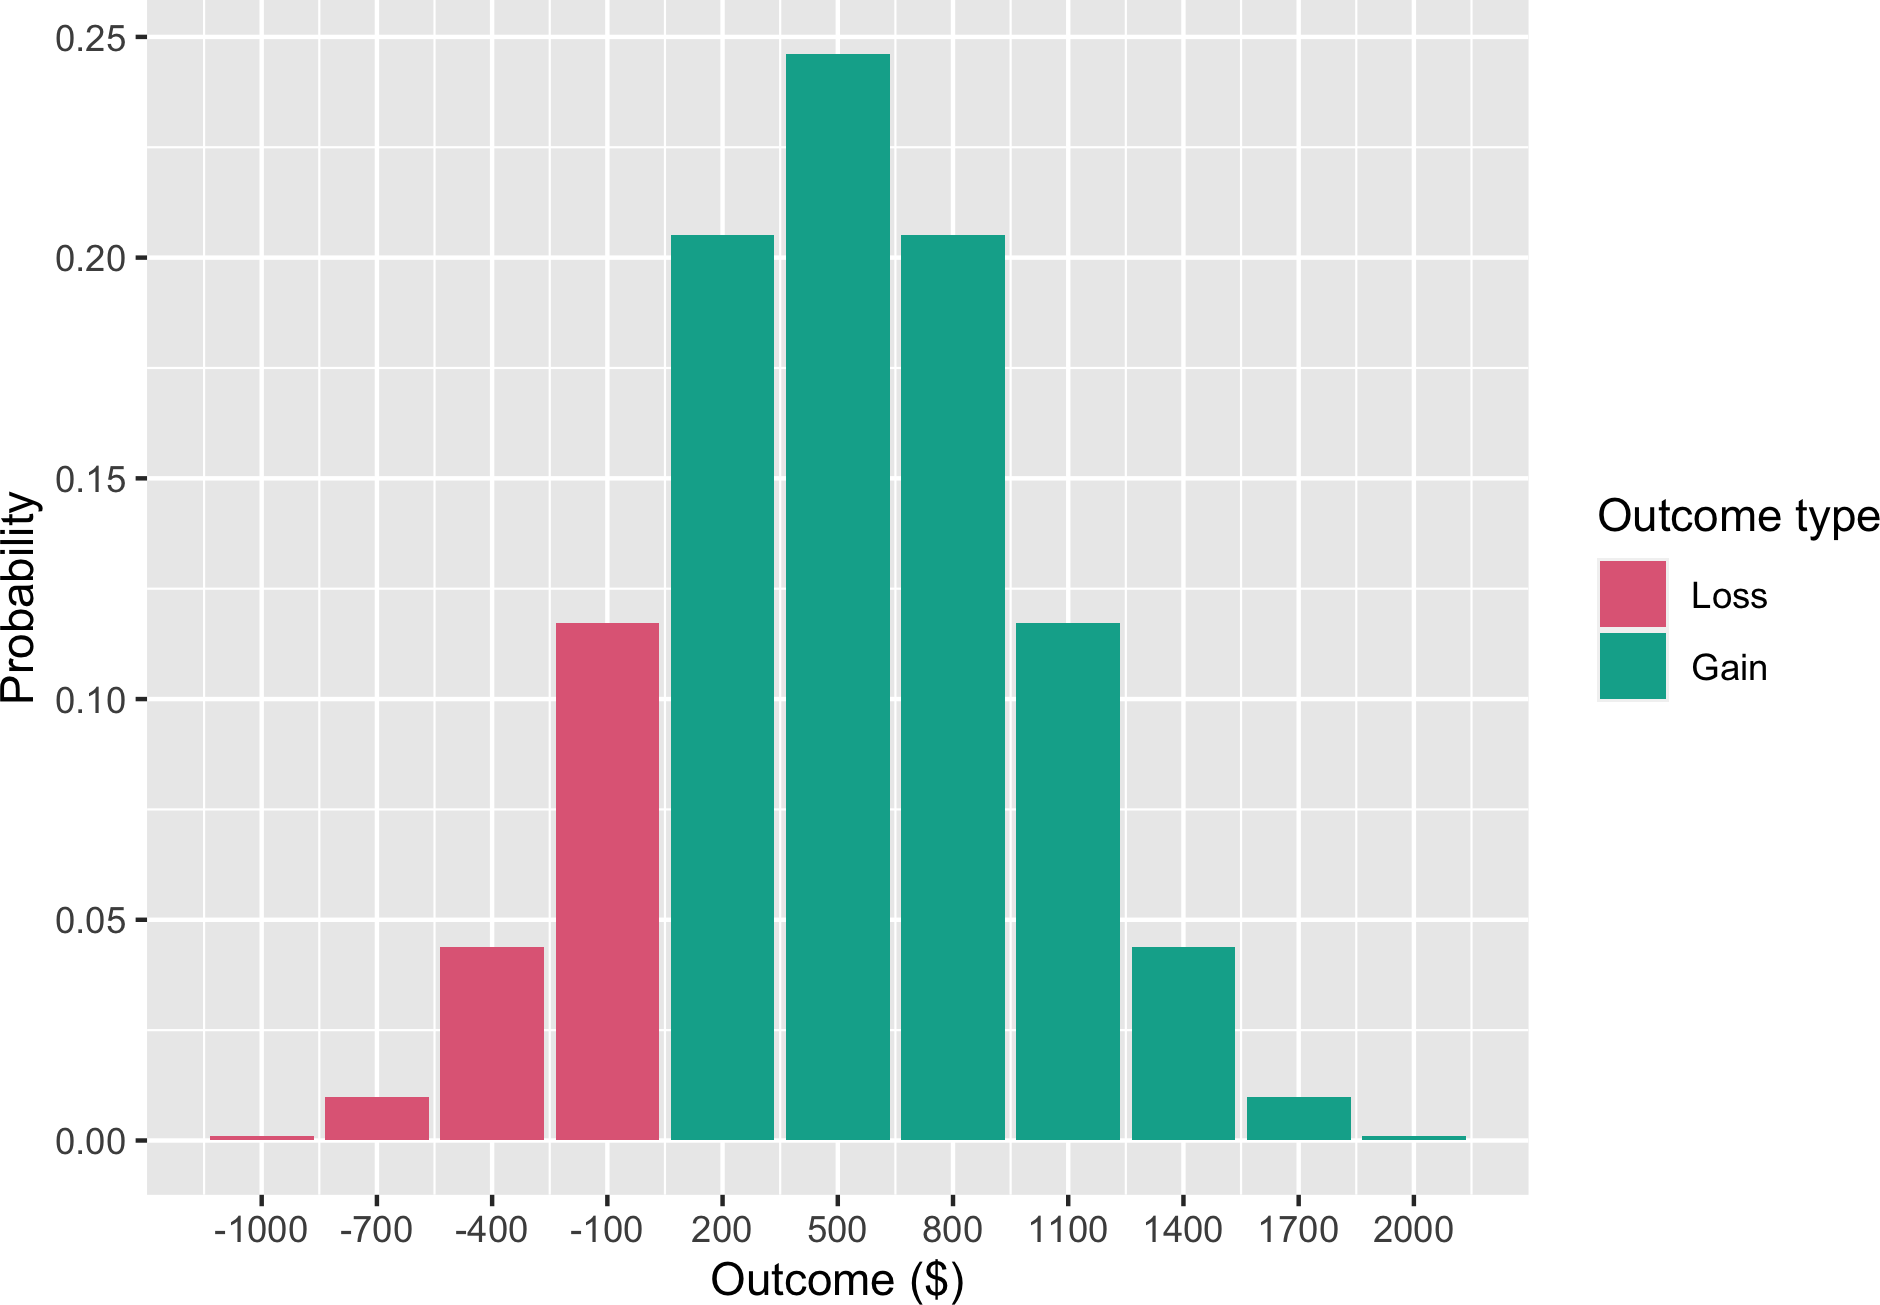
\includegraphics[width=1\linewidth]{effect-of-choice-bracketing-on-risk-aggregation_files/figure-latex/samuelson-distribution-10-1} \caption{The outcome probability distribution of the Samuelson (\protect\hyperlink{ref-samuelson1963}{1963}) gamble (50\% chance of gaining \$200 and a 50\% of losing \$100) played 10 times. Green bars represent gains and red bars represent losses.}\label{fig:samuelson-distribution-10}
\end{figure}

\hypertarget{repeated-play-gambles}{%
\subsubsection{Repeated-Play Gambles}\label{repeated-play-gambles}}

Decisions in real life are usually sequential and rarely identical as in the
multi-play paradigm (cf.~Barron \& Erev, \protect\hyperlink{ref-barron2003}{2003}). That is, people tend to be confronted
with individual choices whose outcomes and outcome probabilities are different
from one choice to another and these choices occur at different points in time.
In a business setting this can be seen in decisions about whether to invest in
new projects; proposals and opportunities differ widely and occur at different
times. Managers are never simply asked: ``here are 10 identical investments to
consider; do you want all or none of them?''

In \emph{repeated-play} (rather than multi-play) gamble paradigms, participants make
decisions about a series of individual gambles. Research using this paradigm
found that people are less risk averse both when outcomes for a series of
gambles are evaluated less frequently and the subsequent decisions are made less
frequently (Bellemare et al., \protect\hyperlink{ref-bellemare2005}{2005}; Beshears et al., \protect\hyperlink{ref-beshears2016}{2016}; Gneezy \& Potters, \protect\hyperlink{ref-gneezy1997}{1997}; Thaler et al., \protect\hyperlink{ref-thaler1997}{1997}). People are
also less risk averse (for positive EV gambles) when they receive feedback after
each decision or are able to sample from the distribution of possible outcomes
before making a choice (Barron \& Erev, \protect\hyperlink{ref-barron2003}{2003}; Camilleri \& Newell, \protect\hyperlink{ref-camilleri2013}{2013}, \protect\hyperlink{ref-camilleri2011}{2011}; Hertwig et al., \protect\hyperlink{ref-hertwig2004}{2004}; Jessup et al., \protect\hyperlink{ref-jessup2008}{2008}; Ludvig \& Spetch, \protect\hyperlink{ref-ludvig2011}{2011}; Wulff et al., \protect\hyperlink{ref-wulff2018}{2018}). Other work found that loss aversion is
mitigated when people are explicitly instructed to consider the options as a
part of a portfolio (Sokol-Hessner et al., \protect\hyperlink{ref-sokolhessner2012}{2012}, \protect\hyperlink{ref-sokolhessner2009}{2009}).

These studies are closer to real-life decisions than the multi-play gamble
paradigm because they involve a set of separate gamble decisions rather than a
single decision about a set of gambles. However, for the most part, the
experiments used in the repeated-play gamble literature use various forms of
feedback throughout the course of the experiment. That is, participants are
shown the outcomes of their gambles before they make more decisions. This
paradigm is known as \emph{experience-based choice}. In \emph{description-based choice},
on the other hand, the gamble is simply presented to the participant without any
feedback, as in the multi-play gambles above. In real life, people rarely see
the immediate outcomes of their risky choices, and even less so in business
settings, where any return on investment often takes years to manifest.

Only a limited number of studies have used a repeated-play paradigm without
feedback. For instance, Jessup et al. (\protect\hyperlink{ref-jessup2008}{2008}) and Hertwig et al. (\protect\hyperlink{ref-hertwig2004}{2004}) investigated the effects of
feedback in repeated-play gambles on the weighting of small probabilities, and
had a no-feedback control condition. Other work similarly used individual
description-based gambles presented sequentially (e.g., Ert \& Erev, \protect\hyperlink{ref-ert2013}{2013}; Joag et al., \protect\hyperlink{ref-joag1990}{1990}).
However, these studies did not attempt to facilitate participants' risk
aggregation. Haisley et al. (\protect\hyperlink{ref-haisley2008}{2008}) provided limited evidence for facilitating risk
aggregation. They gave participants the opportunity to buy five (negative EV)
lottery tickets, and either presented them one at a time, or together.
Participants bought fewer tickets, when they considered them jointly, thereby
maximising EV. However, the experimenters did not specify the outcomes and
probabilities of each gamble, meaning that it is unclear if participants
understood the independent lotteries as identical or non-identical. This reduces
the external validity of the study, as most independent risky choice involves
non-identical outcomes and probabilities. In sum, these studies were not
designed to research how to facilitate risk aggregation and reduce loss
aversion. The experiments in this chapter are novel because their goal is to
facilitate risk aggregation without the experimental artefact of immediate
feedback.

\hypertarget{choice-bracketing}{%
\subsubsection{Choice Bracketing}\label{choice-bracketing}}

Research in psychology and economics has identified ways of facilitating risk
aggregation by encouraging people to group their choices. Specifically, people
aggregate more when they consider the consequences of their choices together
(broad bracketing) than when they consider them individually (narrow
bracketing; Read et al., \protect\hyperlink{ref-read1999}{1999}). In multi-play gambles (especially when displayed with
an outcome distribution), choices are inherently bracketed broadly because a
single choice is made about multiple gambles. Similarly, studies that used
repeated-play gambles facilitated risk-tolerance through what can in hindsight
be considered broad bracketing. For instance, when Thaler et al. (\protect\hyperlink{ref-thaler1997}{1997}) presented gamble
outcomes less frequently, they allowed participants to consider longer time
increments with a single evaluation.

Both the original Samuelson (\protect\hyperlink{ref-samuelson1963}{1963}) anecdote and its subsequent replications show
that people do have an intuition for aggregation even without the risk being
calculated exactly for them. This chapter tests whether that same intuition can
be elicited and applied across sets of unique bets. What are the minimal
conditions required to encourage aggregation? The multi-play gamble work
suggests that participants can engage in a more intuitive form of aggregation
when provided with the right contextual cues. Investigating the effects of more
subtle cues will help shed light on the cognitive processes underlying choice
bracketing. Of course, the effects of more subtle cues would not eliminate the
utility of explicit financial education, but they will help the design of
decision-making contexts to best align with such instruction.

One way of potentially facilitating risk aggregation is to highlight to
participants the number of total options that are available to them.
Sokol-Hessner et al. (\protect\hyperlink{ref-sokolhessner2009}{2009}) and Sokol-Hessner et al. (\protect\hyperlink{ref-sokolhessner2012}{2012}) reduced risk aversion using lengthy
instructions that encouraged participants to ``think like a trader''. This meant
considering all the repeated-play gambles as a portfolio, as opposed to
considering them individually. However, this was quite a strong manipulation
that is perhaps unrealistic in real world. A more subtle cue could involve
simply making participants aware that they are going to be making a series of
choices. If people possess an intuitive understanding of aggregation, as
suggested above, then this kind of contextual cue will also facilitate
aggregation.

In addition to simply informing participants that they will make a series of
choices, making the choices more readily comparable may facilitate broad
bracketing, and thus risk aggregation. Consider the inverse situation wherein a
lack of comparability between choices may prevent broad bracketing, such as when
an executive for a multi-business firm makes decisions across multiple distinct
industries. Of course, the similarity of decision contexts does not change the
maths of risk aggregation, but may well affect whether people do aggregate risk
across decisions. DeKay and Kim (\protect\hyperlink{ref-dekay2005}{2005}) found that multi-play effects are not seen when
choices are not considered fungible. For instance, participants aggregated
across dollar amounts, but not across patients in a medical decision. Therefore,
people may behave similarly when considering a set of dissimilar choices if they
do not consider them fungible.

There is further suggestive evidence that the similarity of a set of choices to
one another will affect choice bracketing. Choices whose differences are easy to
compare (alignable differences) are weighted heavier than those that are
difficult to compare (Markman \& Loewenstein, \protect\hyperlink{ref-markman2010}{2010}; Markman \& Medin, \protect\hyperlink{ref-markman1995}{1995}). Increased similarity across a
set of choices may both highlight the ability for those choices to be bracketed,
and further facilitate risk aggregation through the comparable attributes.
However, it is possible that increased similarity will facilitate risk
aggregation even without a tangible benefit to the underlying calculations. That
is, it is possible that simply manipulating the similarity of
financially-irrelevant semantics of a choice set will make people less risk
averse. If so, then this will be by virtue of an implicit risk aggregation in
which the mere awareness of the possibility of a grouping of choices reduces
risk aversion. It is important to investigate the effect of similarity
especially because in managerial settings, executives in multi-business firms
will often have to make comparisons across industries that are hard to compare.
For instance, GE currently develops both analytic software products and jet
engines for the military. They had been even more diversified previously, at one
stage simultaneously developing home appliances and owning the NBC television
network.

In addition to the similarity between choices, how choices are presented may
affect how easily they are compared, and thus whether or not the multiple
subsequent effects listed above would come to fruition. As mentioned above,
Haisley et al. (\protect\hyperlink{ref-haisley2008}{2008}) found a higher degree of EV maximisation when gambles were
presented jointly, rather than separately. Similarly, Hsee et al. (\protect\hyperlink{ref-hsee1999}{1999}) found that
people's choices were affected by whether they viewed the attributes of the
choices separately or jointly. Their \emph{evaluability hypothesis} suggests that
attributes that are difficult to evaluate will have a greater impact on joint
presentation than separate presentation. Joint presentation is a form of broad
bracketing because it forces a participant to view of all the components of a
decision together. Participants may therefore be more likely to consider
aggregating the risk involved in a set of choices when all those choices are in
view. Joint presentation potentially reduces the working memory load otherwise
needed to maintain that set of choices. Therefore, it is quite possible that a
combination of highly similar choices, presented jointly will lead to the
highest likelihood of broad bracketing, and thus risk aggregation.

Moher and Koehler (\protect\hyperlink{ref-moher2010}{2010}) replicated Gneezy and Potters (\protect\hyperlink{ref-gneezy1997}{1997}), but separately manipulated the number of
gambles seen per trial and feedback frequency. They found that participants were
less risk averse when viewing a set of three gambles per trial, than when
viewing only one. However, they only found this effect with a set of identical
outcomes. When outcomes were non-identical, there was no effect of presentation.
However, participants were always presented with gamble outcomes for each trial,
so it is unclear to what extent this influenced participants' ability to bracket
broadly. In fact, when seeing gambles separately, participants were less risk
averse when receiving feedback for each trial, compared to every three trials.
Testing a presentation manipulation without the confound of feedback will help
to clarify this effect.

\hypertarget{internal-capital-market-investment-context}{%
\subsubsection{Internal Capital Market Investment Context}\label{internal-capital-market-investment-context}}

Executives of large, successful firms are often viewed as fearless risk-takers
who take on risky projects to generate innovation and growth. However, the
available evidence suggests that executives do not view themselves that way
(March \& Shapira, \protect\hyperlink{ref-march1987}{1987}; Swalm, \protect\hyperlink{ref-swalm1966}{1966}). Executives typically evaluate multiple investments
over time. Risk aggregation is sensible when investments are only partially
correlated (i.e., the success of one does not influence the success of another).
It is sensible to take on a set of risky investments with positive EV, where
each investment has some chance of loss, because those that succeed will make up
for those that failed. These benefits are well-known in stock market investment
settings, thanks to Nobel laureate Harry Markowitz's work on modern portfolio
theory (\protect\hyperlink{ref-markowitz1952}{1952}).

However, it is unclear whether the general public and even business managers use
this concept, due to the extent of risk aversion in both those populations
(e.g., Tversky \& Kahneman, \protect\hyperlink{ref-tversky1992}{1992}; March \& Shapira, \protect\hyperlink{ref-march1987}{1987}). In fact, executives treat risk like the rest
of us; they view investments one at a time, are risk averse in the domain of
gains, and are risk seeking in the domain of losses (Lovallo et al., \protect\hyperlink{ref-lovallo2020}{2020}; MacCrimmon et al., \protect\hyperlink{ref-maccrimmon1986}{1986}; Swalm, \protect\hyperlink{ref-swalm1966}{1966}). However, it is understandable why risk aggregation is
foreign to most people; outside of an investment portfolio selection situation,
it is unlikely for people to spontaneously group a selection of individual risky
choices. Usually in life, people encounter risky choices sequentially, and so
the risk of each individual choice is more salient than the aggregated risk of
an arbitrary combination of choices.

Lovallo et al. (\protect\hyperlink{ref-lovallo2020}{2020}) showed that executives treat investments within their own company
in isolation. In multi-business firms, the managers of each business unit often
make the investment decisions about individual projects. Therefore, they often
do not consider the scope of their decisions in the context of the entire
company. For instance, Nobel laureate Richard Thaler offered 25 division
managers working for the same firm a hypothetical investment that involves a 50\%
chance of gaining \$2 million for the company and a 50\% chance of losing \$1
million (\protect\hyperlink{ref-thaler1999}{1999}). Only three managers said they would accept the
investment. However, the CEO indicated that he would have clearly preferred
managers to accept all the investments. To each middle-manager, the choice
represents a risk of loss for their division and potentially their job, whereas
for the CEO the entire portfolio of choices represents a worthwhile risk.

This chapter investigates risky choice in the context of business project
investment internal to a company because this is a real-world context where
choice bracketing is important and currently under-appreciated (Lovallo et al., \protect\hyperlink{ref-lovallo2020}{2020}).
The participants in these experiments were taken from a population that does not
have extensive managerial experience. However, in such a population a lack of
risk aggregation is most likely more common, and the variables used here are
readily applicable to the financial decisions that laypeople make. For instance,
one of the real-world applications of the choice bracketing literature has been
to use outcome distributions and increased time horizons to encourage investment
in high risk, but high EV, retirement funds (e.g., Benartzi \& Thaler, \protect\hyperlink{ref-benartzi1999}{1999}). Otherwise,
people typically prefer low risk, low EV, funds. Further, using laypeople
eliminates potential differences in prior experience with the management-based
decision-context. Upcoming research will focus on managers with context-specific
experience to investigate the effects of that experience.

\hypertarget{aggregation-1}{%
\subsection{Experiment~1}\label{aggregation-1}}

Experiment~1 investigated the effect of three choice bracketing manipulations on
risky choice in hypothetical capital allocation scenarios. Previous research
had low ecological validity because of the use of multi-play paradigms or
feedback. In this experiment, the risky choice task was a description-based
repeated-play paradigm. This means that participants had to make a choice about
whether to accept a number of different hypothetical investments, but were not
provided with the outcome of their choices after each decision. The variables of
interest were the similarity of the choices, whether the choices were presented
together or separately, and whether participants were aware of the number of
choices that they would be making.

The values and probabilities of the gambles were set up such that each
individual gamble, as well as the aggregation of all the gambles, would be
attractive to a rational agent interested in maximising EV. As such, the key
dependent measure was the proportion of risky choices participants accepted.

Previous research suggests that people will be willing to make more risky
choices when explicitly told to bracket their choices (Sokol-Hessner et al., \protect\hyperlink{ref-sokolhessner2012}{2012}, \protect\hyperlink{ref-sokolhessner2009}{2009}). Therefore, Experiment~1 tested the following hypothesis:

\begin{hypothesis}[awareness main effect]
\protect\hypertarget{hyp:awareness-aggregation-1}{}{\label{hyp:awareness-aggregation-1} \iffalse (awareness main effect) \fi{} }Participants that know how many projects to expect will make more risky choices
than participants that are unaware.
\end{hypothesis}

Further, previous work suggests that joint presentation is a form of broad
bracketing (e.g., Moher \& Koehler, \protect\hyperlink{ref-moher2010}{2010}; Hsee et al., \protect\hyperlink{ref-hsee1999}{1999}). Therefore, Experiment~1 tested the
following hypothesis:

\begin{hypothesis}[presentation main effect]
\protect\hypertarget{hyp:presentation-aggregation-1}{}{\label{hyp:presentation-aggregation-1} \iffalse (presentation main effect) \fi{} }Participants will make more risky choices when seeing projects jointly than when
seeing them separately.
\end{hypothesis}

Similarity of options has also been shown to affect the way people bracket their
choices (e.g., DeKay \& Kim, \protect\hyperlink{ref-dekay2005}{2005}). Therefore, Experiment~1 tested the following hypothesis:

\begin{hypothesis}[similarity main effect]
\protect\hypertarget{hyp:similarity-aggregation-1}{}{\label{hyp:similarity-aggregation-1} \iffalse (similarity main effect) \fi{} }Participants that see projects from the same industry will make more risky
choices than participants that see projects from different industries.
\end{hypothesis}

\hypertarget{method}{%
\subsubsection{Method}\label{method}}

\hypertarget{participants}{%
\paragraph{Participants}\label{participants}}

One hundred and ninety-eight participants (82 female) were recruited from the online recruitment platform Prolific. Participants were compensated at a rate of \pounds 5 an hour (Prolific is based in the UK). The average age was 32.52 years (\emph{SD} = 11.42, \emph{min.} = 18, \emph{max.} = 69). Participants reported an average of 7.01 years (\emph{SD} = 9.1, \emph{min.} = 0, \emph{max.} = 42) working in a business setting, and an average of 1.7 years (\emph{SD} = 2.85, \emph{min.} = 0, \emph{max.} = 20) of business education. The mean completion time of the task was 12.04 min (\emph{SD} = 11.29, \emph{min.} = 3.1, \emph{max.} = 112.4).~Table~\ref{tab:condition-allocation-aggregation-1}
shows the allocation of participants to the different conditions.

\begin{table}[tbp]

\begin{center}
\begin{threeparttable}

\caption{\label{tab:condition-allocation-aggregation-1}Experiment 1 group allocation.}

\begin{tabular}{lll}
\toprule
Similarity & \multicolumn{1}{c}{Awareness} & \multicolumn{1}{c}{N}\\
\midrule
High & Aware & 53\\
High & Naive & 53\\
Low & Aware & 47\\
Low & Naive & 45\\
Total &  & 198\\
\bottomrule
\end{tabular}

\end{threeparttable}
\end{center}

\end{table}

\hypertarget{materials}{%
\paragraph{Materials}\label{materials}}

\hypertarget{instructions-materials-aggregation-1}{%
\subparagraph{Instructions}\label{instructions-materials-aggregation-1}}

Participants were told to imagine that they are executives in a large company
and that they will need to decide about investing in a number of hypothetical
business projects. The appendix shows these instructions in
Figure~\ref{fig:instructions-materials-aggregation-1}.

\hypertarget{task-aggregation-1}{%
\subparagraph{Risky Investment Task}\label{task-aggregation-1}}

Participants saw 10 short descriptions of business projects, and were asked
whether they would invest in that project or not. Each description included the
name of the hypothetical business, the amount they forecast the project to cost,
the amount the project is forecast to make, and probabilities for these
forecasts. The project values were selected so that the projects appeared
attractive when aggregated, and unattractive when segregated (see Langer \& Weber, \protect\hyperlink{ref-langer2001}{2001}).
These values were different for each project, but followed a set of constraints
for each project's EV and the probability of any loss given the outcome
distribution of all 10 projects (\(P(\text{loss}_{aggregated})\)). Further, there
was a constraint on the gambles' loss aversion coefficient (\(\lambda\)), which is
a measure of people's sensitivity to losses compared to gains. The constraints
were:

\begin{enumerate}
\def\labelenumi{\arabic{enumi}.}
\item
  \(\text{EV} > 0\);
\item
  \(\lambda < 2.25\); and
\item
  \(P(\text{loss}_{aggregated}) < 0.1\).
\end{enumerate}

As such, each project cannot be considered to be a loss in terms of expected
value, but also would not be an easy choice for investment, because of the low
\(\lambda\) (made to be lower than the median loss aversion coefficient calculated
in Tversky \& Kahneman, \protect\hyperlink{ref-tversky1992}{1992}). Further, since people are especially sensitive to loss
probabilities (Kahneman \& Tversky, \protect\hyperlink{ref-kahneman1979}{1979}; Zeisberger, \protect\hyperlink{ref-zeisberger2020}{2020}), an arbitrarily low
\(P(\text{loss}_{aggregated})\) was chosen to make investment in the complete set
of projects seem attractive. The actual probability of a loss given the outcome
distribution used in the experiment was 0.09.
This was calculated by summing all probabilities in the Poisson binomial
distribution whose outcomes were less than zero. For comparison,
\(P(\text{loss}_{aggregated})\) = 0.17
for 10 plays of the Samuelson (\protect\hyperlink{ref-samuelson1963}{1963}) gamble. The highest probability of a loss for
any single gamble (\(P(\text{loss}_{single})\)) was
0.80.
Figure~\ref{fig:project-choice-aggregation-1} shows an example of a description
of a project in this task.



\begin{figure}
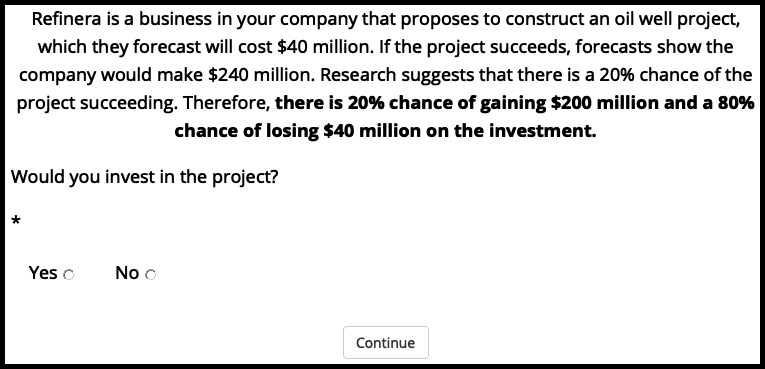
\includegraphics[width=1\linewidth]{effect-of-choice-bracketing-on-risk-aggregation_files/figure-latex/project-choice-aggregation-1-1} \caption{Example of a project choice display in Experiment~1.}\label{fig:project-choice-aggregation-1}
\end{figure}

In the high similarity condition, these project descriptions were all about one
type of project (in this case an oil well project) and were all from the same
business. In the low similarity condition, each project was from a different
industry. In the joint presentation condition, the 10 projects were all
displayed on the one webpage, whereas in the separate presentation condition
each was displayed on a different webpage. Participants in the aware condition
saw the display shown in Figure~\ref{fig:awareness-aware-aggregation-1} before
their separate presentation display. Those in the naive condition simply
proceeded without this message. The financial and probability values were
identical regardless of condition, and the order of each set of 10 projects was
randomised.



\begin{figure}

\includegraphics[width=1\linewidth]{effect-of-choice-bracketing-on-risk-aggregation_files/figure-latex/awareness-aware-aggregation-1-1} \caption{The display seen by those in the aware condition of Experiment~1.}\label{fig:awareness-aware-aggregation-1}
\end{figure}

Although the project descriptions were succinct, and the decisions in the task
were made quickly, they reflect real decisions in businesses in critical ways.
Companies that consider their forecast estimates probabilistically (i.e., do not
simply use the most likely estimate as the only estimate) do frame their options
as likelihoods of certain monetary outcomes.

\hypertarget{outcome-distribution-materials-aggregation-1}{%
\subparagraph{Outcome Distribution Decision}\label{outcome-distribution-materials-aggregation-1}}

Participants were asked if they would invest in the last 10 projects they saw
and were provided with a graph of the outcome probability distribution of the 10
projects. Figure~\ref{fig:project-choice-aggregated-aggregation-1} shows this
graph. A coding error was discovered after collecting data. This was an error in
the generation of gambles, which meant that the outcome distribution decision
data could not be used. Therefore, the effect of outcome distribution will not
be discussed until Experiment~2, which fixed this issue.
Appendix~\ref{outcome-distribution-aggregation-1} presents an analysis of these
data, and describes the coding error and its implications.

\hypertarget{follow-up-gambles}{%
\subparagraph{Follow-up Gambles}\label{follow-up-gambles}}

Participants were shown four further sets of gambles (11 total) that checked
participant attention and replicated the gambles from Samuelson (\protect\hyperlink{ref-samuelson1963}{1963}) and
Redelmeier and Tversky (\protect\hyperlink{ref-redelmeier1992}{1992}). See Appendix~\ref{follow-up-materials-aggregation-1-appendix}
for details.

\hypertarget{procedure}{%
\paragraph{Procedure}\label{procedure}}

Participants read the instructions and completed the risky investment task,
first in the separate presentation condition, and then in the joint condition.
They then made the outcome distribution decision and responded to the 11
follow-up gambles.

\hypertarget{results-aggregation-1}{%
\subsubsection{Results}\label{results-aggregation-1}}

\hypertarget{project-choice}{%
\paragraph{Project Choice}\label{project-choice}}

A three-way analysis of variance (ANOVA) was conducted to investigate the
effects of similarity, awareness, and presentation on the proportion of
participants' decision to invest in the 10 projects. As seen in
Figure~\ref{fig:plot-aggregation-1-awareness}, participants invested more when
they were told that there will be 10 projects, compared with when they were not
told this, \(F(1, 194) = 9.52\), \(p = .002\), \(\hat{\eta}^2_p = .047\). As seen in
Figure~\ref{fig:plot-aggregation-1-presentation}, participants invested more
when viewing the projects jointly, compared with when they viewed them separately,
\(F(1, 194) = 1.54\), \(p = .216\), \(\hat{\eta}^2_p = .008\). Although there was no main effect of
similarity, \(F(1, 194) = 1.63\), \(p = .204\), \(\hat{\eta}^2_p = .008\), the interaction between
similarity and presentation was significant,
\(F(1, 194) = 4.31\), \(p = .039\), \(\hat{\eta}^2_p = .022\) (see
Figure~\ref{fig:plot-aggregation-1-similarity-presentation}). Specifically, the
presentation effect was stronger in the high similarity condition,
\(\Delta M = 0.07\), 95\% CI \([0.04,~0.09]\), \(t(194) = 5.29\), \(p < .001\), than in the low similarity
condition, \(\Delta M = 0.03\), 95\% CI \([0.00,~0.05]\), \(t(194) = 2.06\), \(p = .041\). These findings
suggest that it is possible to facilitate risk aggregation with subtle choice
bracketing manipulations.



\begin{figure}
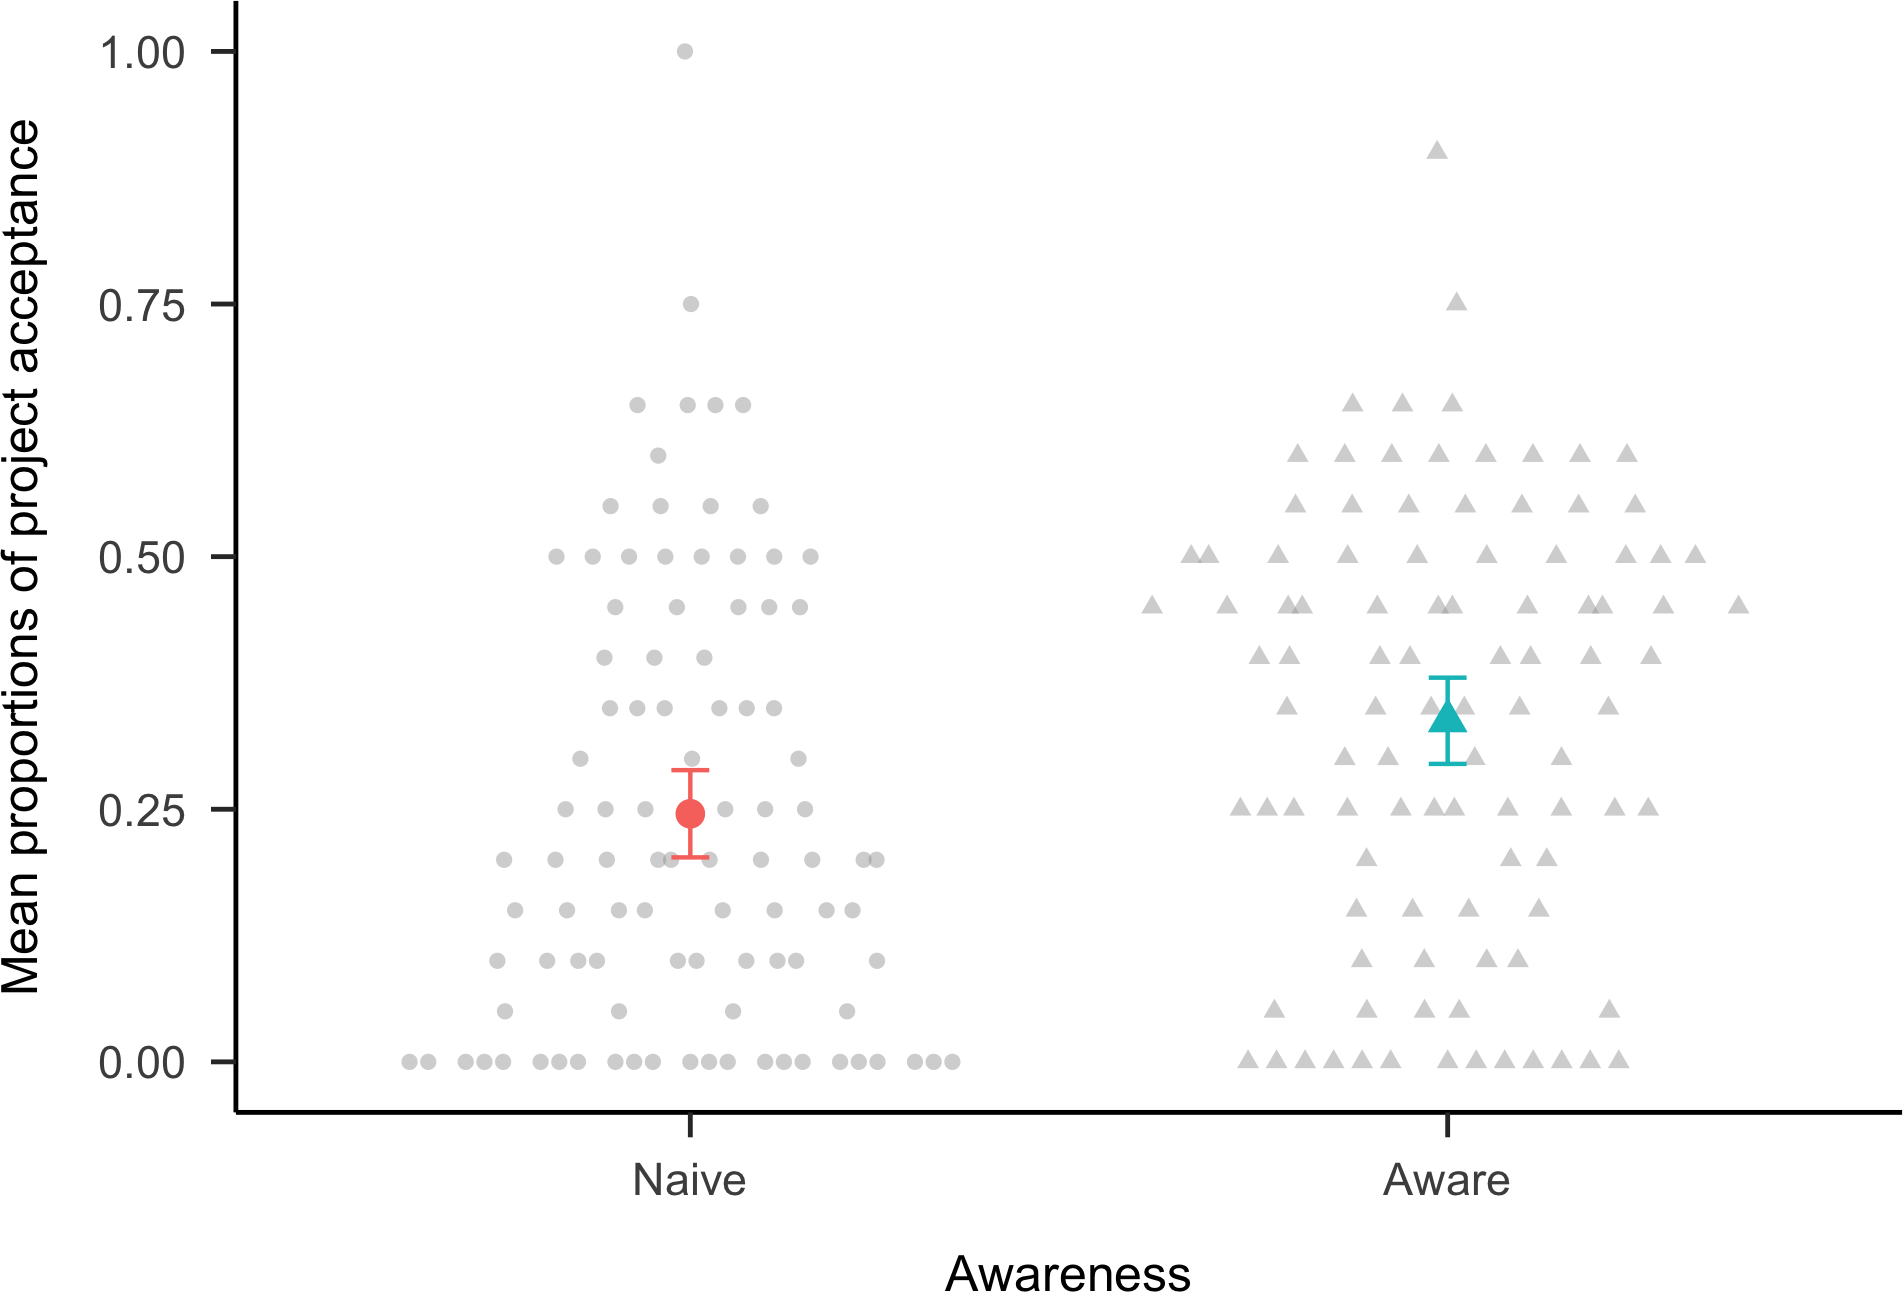
\includegraphics[width=1\linewidth]{effect-of-choice-bracketing-on-risk-aggregation_files/figure-latex/plot-aggregation-1-awareness-1} \caption{Mean proportions of decisions to invest in each set of 10 projects, by awareness condition. Error bars represent 95\% confidence intervals. Raw data are plotted in the background.}\label{fig:plot-aggregation-1-awareness}
\end{figure}



\begin{figure}
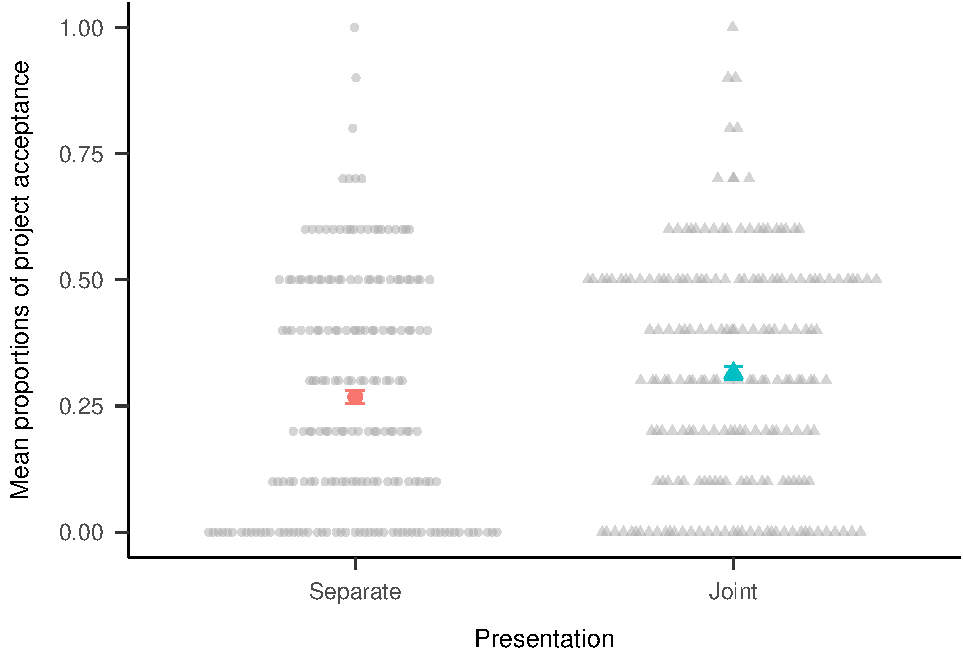
\includegraphics[width=1\linewidth]{effect-of-choice-bracketing-on-risk-aggregation_files/figure-latex/plot-aggregation-1-presentation-1} \caption{Mean proportions of decisions to invest in each set of 10 projects, by presentation condition. Error bars represent 95\% confidence intervals. Here, however, the intervals are so narrow that they are sometimes obscured by the mean indicators in the plot. Raw data are plotted in the background.}\label{fig:plot-aggregation-1-presentation}
\end{figure}



\begin{figure}
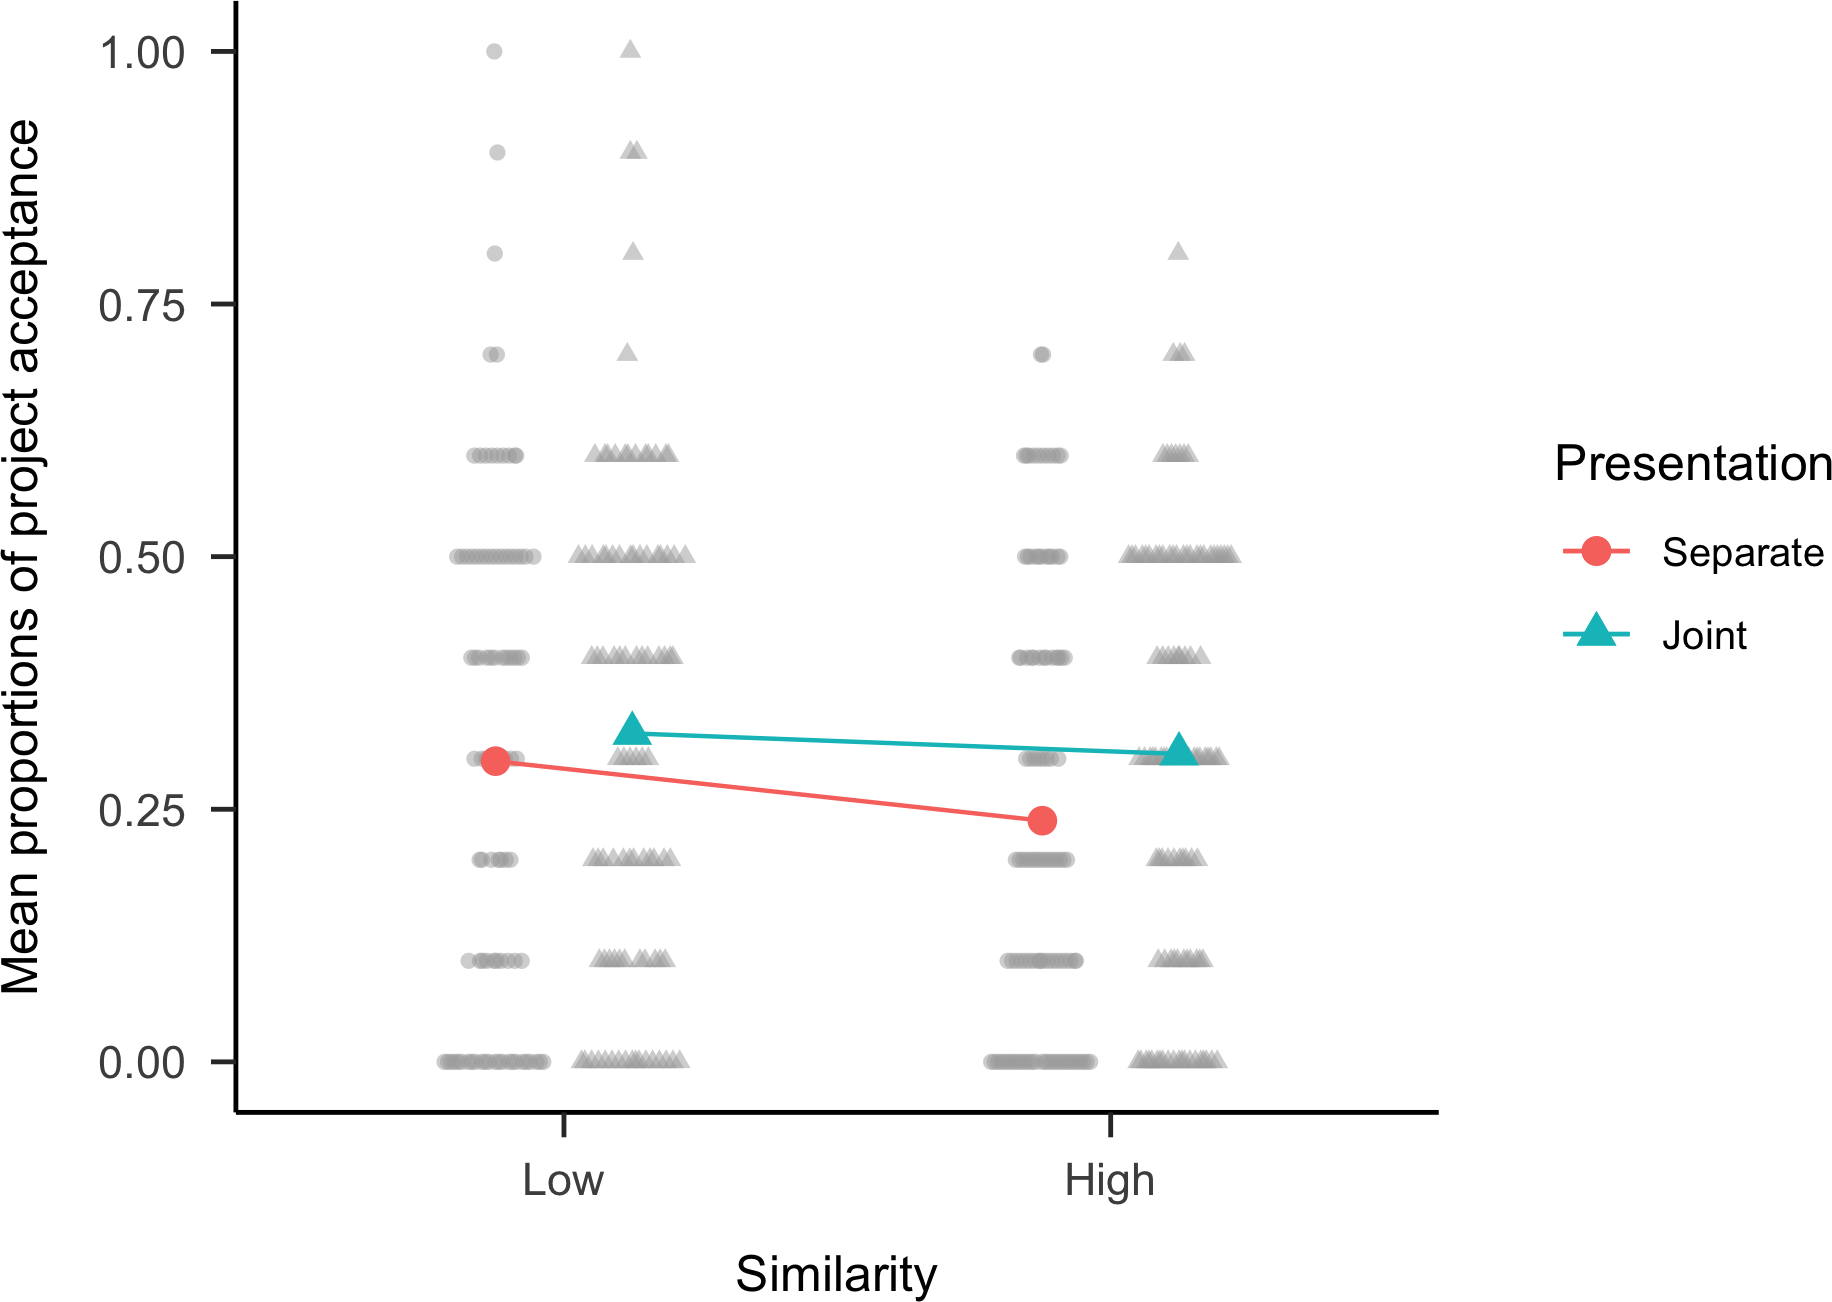
\includegraphics[width=1\linewidth]{effect-of-choice-bracketing-on-risk-aggregation_files/figure-latex/plot-aggregation-1-similarity-presentation-1} \caption{Mean proportions of decisions to invest in each set of 10 projects, by similarity and presentation conditions. In mixed factorial designs, error bars cannot be used to make inferences by ``eye'' across all conditions. Therefore, error bars are not included. Raw data are plotted in the background.}\label{fig:plot-aggregation-1-similarity-presentation}
\end{figure}

\hypertarget{trial-by-trial-analysis}{%
\paragraph{Trial-by-Trial Analysis}\label{trial-by-trial-analysis}}

Exploratory analyses were conducted into the possible effects of the
manipulations on a trial-by trial basis.
Figure~\ref{fig:plot-aggregation-1-trials} shows the data for all conditions.
However, the key findings are in the separate presentation. As
Figure~\ref{fig:plot-aggregation-1-trials-separate-awareness} shows, in the
separate condition people are more likely to accept projects over the 10 trials,
but this interacts with awareness,
\(b = 0.04\), 95\% CI \([0.01, 0.08]\), \(z = 2.32\), \(p = .021\).
Specifically, the relationship between choice and trial is stronger in the aware
condition,
\(b = 0.11\), 95\% CI \([0.06, 0.16]\), \(z = 4.54\), \(p < .001\), than in the
naive condition,
\(b = 0.03\), 95\% CI \([-0.03, 0.08]\), \(z = 1.01\), \(p = .311\). It seems that
participants that were told the total number of projects became less risk averse
as the experiment proceeded, regardless of the gamble values.



\begin{figure}
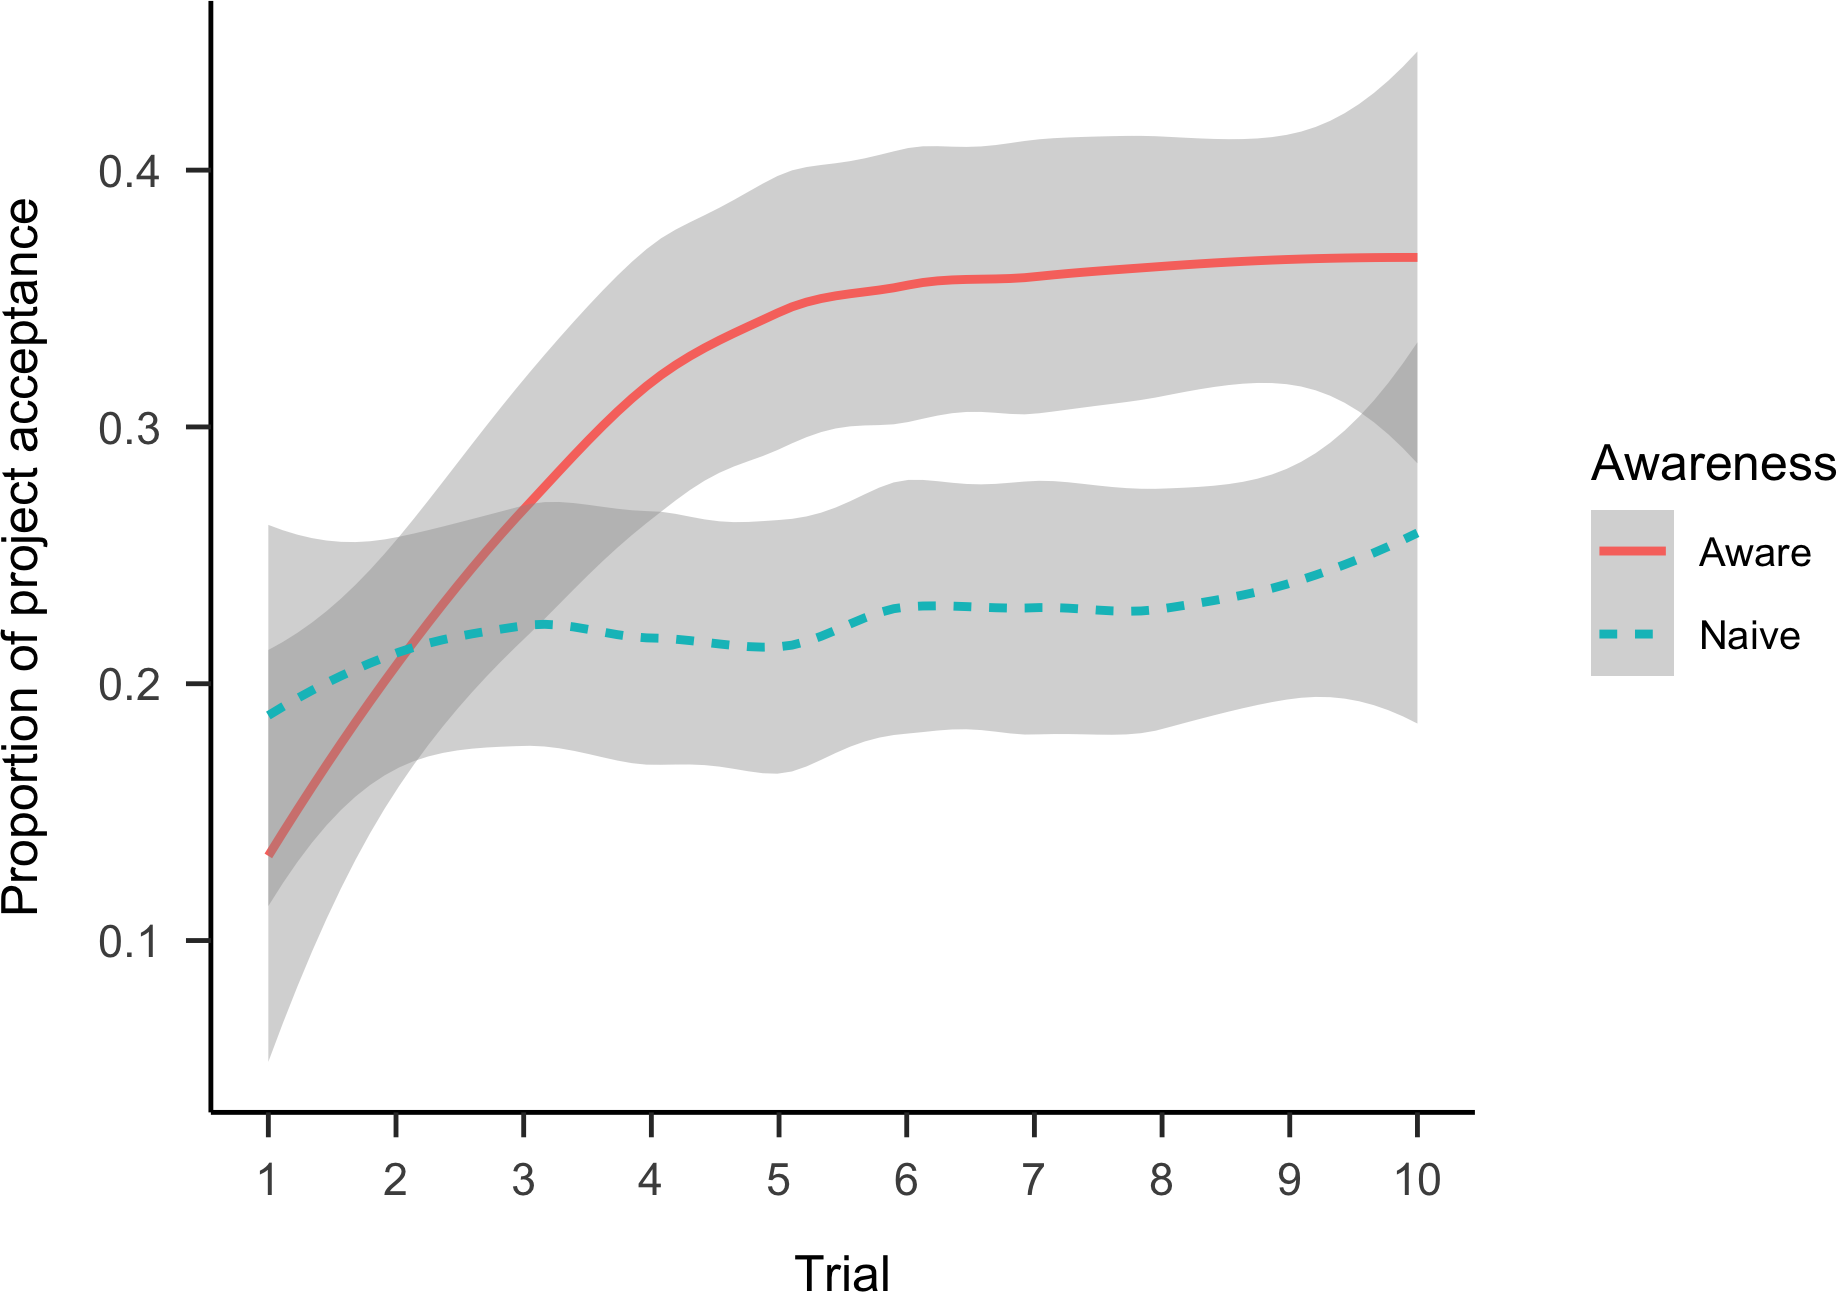
\includegraphics[width=1\linewidth]{effect-of-choice-bracketing-on-risk-aggregation_files/figure-latex/plot-aggregation-1-trials-separate-awareness-1} \caption{Proportion of project acceptance in the separate presentation condition, by trial and awareness conditions. LOESS method was used for smoothing over trials and the shading represents 95\% confidence intervals.}\label{fig:plot-aggregation-1-trials-separate-awareness}
\end{figure}

\hypertarget{discussion-aggregation-1}{%
\subsubsection{Discussion}\label{discussion-aggregation-1}}

Experiment~1 found evidence for most of the hypotheses. Specifically, people
made more risky choices when considering those choices jointly on the same page,
compared to on separate pages; and when they knew how many choices were in the
set. Further, the results showed an interaction between project similarity and
presentation. Exploratory analyses showed that participants' risk aversion
decreased as they proceeded through the trials, but only when participants were
aware of the number of projects.

\hypertarget{presentation-effect}{%
\paragraph{Presentation Effect}\label{presentation-effect}}

The presentation effect may be a result of one of two mechanisms. A mathematical
aggregation explanation would mean that participants are combining the gambles
into a mental representation of the probability distribution and then deciding
based on the attractiveness of that distribution. A joint presentation of
choices would facilitate this combination. On the other hand, people may also be
using a sort of naive aggregation process when they are encouraged to group
their choices together. A naive aggregation explanation would suggest that
participants in the joint condition are simply more likely to realise that a few
big wins could offset a few losses. Participants could have been encouraged by
the joint display to consider the set of projects together. This could then lead
to the conclusion that investing in a higher number of gambles might mean that
the gains of some projects will pay off the losses of the other projects.

\hypertarget{awareness-effect}{%
\paragraph{Awareness Effect}\label{awareness-effect}}

Experiment~1 found that participants that viewed the projects separately were
more likely to invest in the projects as the trials went on, regardless of the
actual gambles. Having an awareness of the total number of projects in the set
could increase the likelihood that participants would naively aggregate.
Specifically, knowing the number of total projects might increase the salience
of the idea that the gains of some projects will offset the losses of others,
because it reinforces a focus on the entire set. Another possibility is that
participants had a certain aspiration level (Lopes, \protect\hyperlink{ref-lopes1996}{1996}) that they were
attempting to reach. This might mean that they invested more as the task
proceeded after realising that the gambles were not becoming significantly more
favourable. Barron and Erev (\protect\hyperlink{ref-barron2003}{2003}, p. 219) specifically did not tell participants about
the number of gambles they would experience to ``avoid an `end of task' effect
(e.g., a change in risk attitude)''. Barron and Erev (\protect\hyperlink{ref-barron2003}{2003}) provided participants with
feedback, but this should not be necessary for an aspiration level explanation
since participants only need to be aware of the potential for certain gains.

This result may also be due to a Gambler's fallacy effect or the law of small
numbers. This effect is characterised by people's expectation of a pattern to
follow the underlying distribution of the function that generates each
component. For instance, someone observing the results of a coin flip that look
like HTTHTTTT might anticipate that the likelihood of ``heads'' is higher than
that of ``tails'', despite the actual likelihood being 50\% for either. This effect
occurs in sequential decision-making, so may be relevant for the repeated-play
decisions in Experiment~1. Barron and Leider (\protect\hyperlink{ref-barron2010}{2010}) found that the gambler's fallacy (in a
roulette prediction task) emerges when information about past outcomes was
displayed sequentially, but not when it is displayed all at once. Haisley et al. (\protect\hyperlink{ref-haisley2008}{2008})
found evidence for the gambler's fallacy with a repeated-play gamble paradigm.
As such, it is possible that an effect such as the Gambler's fallacy can explain
the effect of the awareness manipulation. That is, participants may have thought
that after a few gambles that they considered risky, the last ones were more
likely to materialise. Further, this would be more likely to occur for those
that knew the total number of projects, because they knew when the sequence was
approaching its end.

\hypertarget{similarity-discussion-aggregation-1}{%
\paragraph{Similarity Effect}\label{similarity-discussion-aggregation-1}}

Experiment~1 did not find a main effect of similarity in the individual choice
data as predicted in Hypothesis~\ref{hyp:similarity-aggregation-1}. Instead,
choice similarity interacted with the presentation condition. This interaction
is harder to explain since it was not hypothesised. In fact, the results seem to
suggest the opposite to what was originally expected. Initially, it was
predicted that people would be less risk averse in the high similarity
condition, due to the better ability to consider the isolated projects as a
grouped set. Similarity was thought to act as a broad bracket, and therefore
increase aggregation. That is, it was expected that seeing a set of similar
projects would help participants aggregate risk when seeing them separately,
more than when projects are dissimilar. Instead, project acceptance was actually
numerically higher in the low than in the high similarity condition
(\(\Delta M = -0.06\), 95\% CI \([-0.12,~0.00]\), \(t(194) = -1.82\), \(p = .070\)) when projects were
presented separately, averaging over awareness conditions.

There was no significant difference between similarity conditions regardless of
presentation condition. However, allocations were significantly higher in the
joint presentation condition than in the separate condition for both high and
low similarity. The interaction seems to have been found due to the larger
difference in the high similarity condition. Perhaps the ability to aggregate
risk when projects are presented together is more made more salient when
projects are similar.

Specifically, the interaction seems to be driven by the separate high similarity
condition being lower, rather than by the joint high similarity being higher, as
would have been expected. As such, participants could have been engaged in a
naive \emph{diversification}, rather than a naive aggregation. In ``true''
diversification, people would choose a set of projects that are partially (and
ideally negatively) correlated, as per Markowitz (\protect\hyperlink{ref-markowitz1952}{1952}). However, in reality
people that intend to diversify only seem diversify naively, meaning that they
neglect co-variation when diversifying (e.g., Hedesstrom et al., \protect\hyperlink{ref-hedesstrom2006}{2006}). Instead, they
only seem to be looking for variety, rather than diversification in the strict
sense. This \emph{diversification bias} is also seen in product choices (Read \& Loewenstein, \protect\hyperlink{ref-read1995}{1995}).

In Experiment~1, participants may have considered the high similarity condition
as a sign that the set of projects may not be sufficiently ``diversified''.
However, this explanation would also predict the joint presentation condition to
be lower in the high similarity condition. So, perhaps when in the separate
condition, participants were constantly thinking that they might be getting a
different project in the next display, so rejected more projects because of the
lack of diversification, but not realising that they would not be getting any
other type of project. Those in the joint presentation, on the other hand, were
able to see all ten projects, so already knew that there were no other projects
in the set, and so were less likely to reject projects on the basis of the hope
for different projects in the future.

\hypertarget{limitations}{%
\paragraph{Limitations}\label{limitations}}

This experiment had two major limitations. First, proper counterbalancing was
not used in the high alignment project domain, nor in the order of the
within-subjects manipulation of presentation. As such, it is unclear what role
these elements played in the results, especially in the presentation condition,
in which participants always saw the separate condition first. Second, as
mentioned above in Section~\ref{outcome-distribution-materials-aggregation-1},
there was a mistake in the generation of the gamble values that meant that the
individual gambles did not correspond with the distribution that participants
saw. Both of these limitations were addressed in Experiment~2.

\hypertarget{aggregation-2}{%
\subsection{Experiment~2}\label{aggregation-2}}

Experiment~2 investigated the effect of presentation, awareness, and
distribution on project choice. For the distribution manipulation, half of the
sample saw an outcome probability distribution as in the previous literature
(e.g., Redelmeier \& Tversky, \protect\hyperlink{ref-redelmeier1992}{1992}; Webb \& Shu, \protect\hyperlink{ref-webb2017}{2017}) to determine their risk aversion when the
gambles are explicitly aggregated. In contrast to most of the repeated-play
choice literature, each choice was presented without subsequent feedback.
Further, in contrast to Experiment~1, the distribution was displayed alongside
each gamble, as opposed to only at the very end. This is an important
manipulation because finding out whether it is effective will (a) add to the
understanding of the conditions necessary for mathematical aggregation (beyond a
mere intuitive sense of aggregation), and (b) suggest new ways to encourage
aggregation in real-world applications.

In past work, participants were shown ordinary binomial distributions, since
multi-play gambles are identical. However, there has not been an investigation
of \emph{non-identical} gamble distributions in this context. Doing this requires
using a \emph{Poisson} binomial distribution, which allows for multiple trials with
different probabilities.

Further, Experiment~2 addressed potential order effects in Experiment~1 by
manipulating all the main variables between-subjects. Manipulating presentation
between-subjects, removes the potentially confounding factor of reduced risk
aversion over time.

Experiment~2 again tested Hypotheses~\ref{hyp:awareness-aggregation-1},
and~\ref{hyp:presentation-aggregation-1}, from Experiment~1. Further, following
the finding in Experiment~1 that participants in the aware condition seemed to
become more risk-taking as the experiment progressed, Experiment~2 tested the
following hypothesis:

\begin{hypothesis}[interaction of trial number and awareness]
\protect\hypertarget{hyp:awareness-trials-aggregation-2}{}{\label{hyp:awareness-trials-aggregation-2} \iffalse (interaction of trial number and awareness) \fi{} }Participants will make more risky choices as the trials progress, but only when
they are aware of the total number of projects in the set.
\end{hypothesis}

Further, multi-play gambles with outcome distributions have been shown to reduce
risk aversion compared to multi-play gambles without distributions (e.g., Redelmeier \& Tversky, \protect\hyperlink{ref-redelmeier1992}{1992}; Webb \& Shu, \protect\hyperlink{ref-webb2017}{2017}). Therefore, Experiment~2 tested the following
hypothesis:

\begin{hypothesis}[distribution effect]
\protect\hypertarget{hyp:distribution-aggregation-2}{}{\label{hyp:distribution-aggregation-2} \iffalse (distribution effect) \fi{} }Participants will make more risky choices when presented with an aggregated
outcome distribution than when making the same decisions individually.
\end{hypothesis}

\hypertarget{method-1}{%
\subsubsection{Method}\label{method-1}}

\hypertarget{participants-1}{%
\paragraph{Participants}\label{participants-1}}

One hundred and sixty-four participants (51 female) were recruited from the online recruitment platform Prolific. Participants were compensated at a rate of \pounds 5 an hour (Prolific is based in the UK). The average age was 26.39 years (\emph{SD} = 8.63, \emph{min.} = 18, \emph{max.} = 72). Participants reported an average of 2.55 years (\emph{SD} = 5.34, \emph{min.} = 0, \emph{max.} = 43) working in a business setting, and an average of 1.67 years (\emph{SD} = 2.94, \emph{min.} = 0, \emph{max.} = 20) of business education. The mean completion time of the task was 6.53 min (\emph{SD} = 5.15, \emph{min.} = 1.18, \emph{max.} = 39.93).~Table~\ref{tab:condition-allocation-aggregation-2}
shows the allocation of participants to the different conditions.
Appendix~\ref{power-analysis-aggregation-2} describes the power analysis
conducted to arrive at this sample size.

\begin{table}[tbp]

\begin{center}
\begin{threeparttable}

\caption{\label{tab:condition-allocation-aggregation-2}Experiment 2 group allocation.}

\begin{tabular}{llll}
\toprule
Awareness & \multicolumn{1}{c}{Distribution} & \multicolumn{1}{c}{Presentation} & \multicolumn{1}{c}{N}\\
\midrule
Aware & Absent & Separate & 40\\
Naive & Absent & Joint & 41\\
Naive & Absent & Separate & 41\\
Naive & Present & Separate & 42\\
Total &  &  & 164\\
\bottomrule
\end{tabular}

\end{threeparttable}
\end{center}

\end{table}

\hypertarget{materials-1}{%
\paragraph{Materials}\label{materials-1}}

\hypertarget{instructions}{%
\subparagraph{Instructions}\label{instructions}}

Participants were shown the same instructions as in Experiment~1 (see
Section~\ref{instructions-materials-aggregation-1}).

\hypertarget{task-aggregation-2}{%
\subparagraph{Risky Investment Task}\label{task-aggregation-2}}

Participants saw a similar display to the one in Experiment~1 (see
Section~\ref{task-aggregation-1}), but with new gamble values, in order to fix
the mistake in the Experiment~1 gamble value calculation (detailed in the
appendix Section~\ref{outcome-distribution-aggregation-1}).

The presentation and awareness manipulations were as in Experiment~1. However,
in the distribution-present condition participants saw the outcome probability
distribution of all the projects alongside the description, rather than after
all the projects were seen (see
Figure~\ref{fig:separate-distribution-present-aggregation-2}).



\begin{figure}
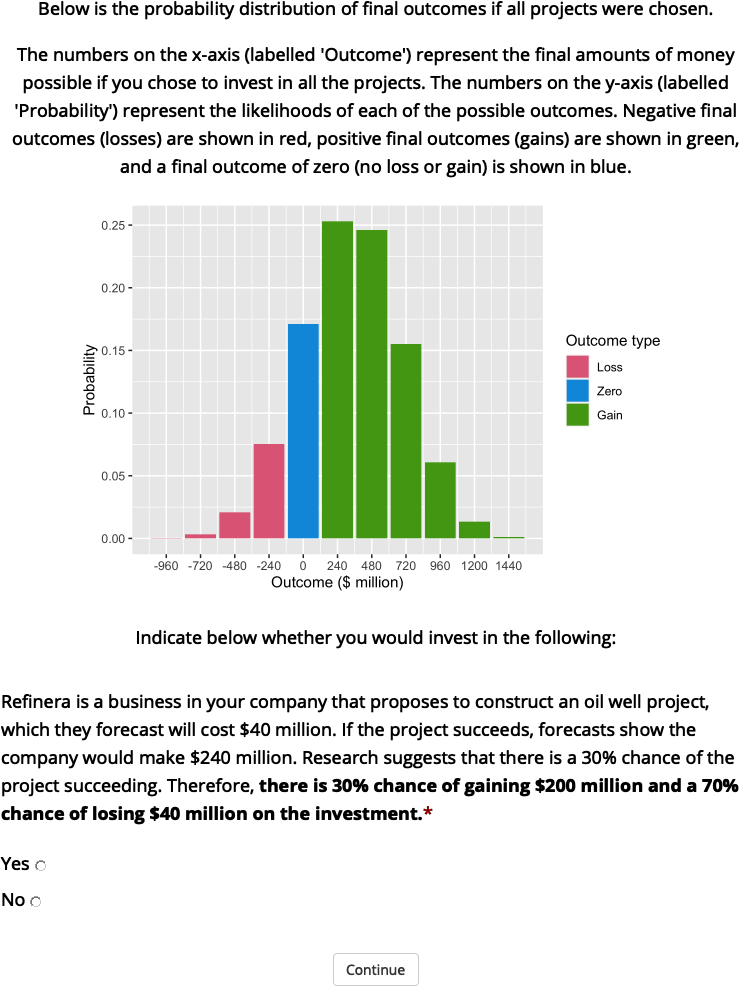
\includegraphics[width=1\linewidth]{effect-of-choice-bracketing-on-risk-aggregation_files/figure-latex/separate-distribution-present-aggregation-2-1} \caption{An example of a display seen by those in the separate distribution-present condition of Experiment~2.}\label{fig:separate-distribution-present-aggregation-2}
\end{figure}

\hypertarget{follow-up-aggregation-2}{%
\subparagraph{Follow-up}\label{follow-up-aggregation-2}}

Participants were asked how many projects they thought they saw, whether they
were willing to accept all or none of the projects, and how many they would be
willing to accept if they had to choose a number.
Appendix~\ref{follow-up-materials-aggregation-2-appendix} shows these
questions.

\hypertarget{procedure-1}{%
\paragraph{Procedure}\label{procedure-1}}

Participants read the instructions and completed the risky investment task in
their respective conditions. After seeing the individual projects, participants
were then asked the three follow-up questions.

\hypertarget{results-aggregation-2}{%
\subsubsection{Results}\label{results-aggregation-2}}

\hypertarget{project-investment}{%
\paragraph{Project Investment}\label{project-investment}}

The project investment data were analysed as proportions of choice per
participant, as in Experiment~1. Each experimental condition was compared to the
same control condition (separate presentation, naive awareness, and distribution
absent). Figure~\ref{fig:plot-aggregation-2-proportion} shows these data. The
difference between presentation conditions was not significant,
\(F(1, 80) = 0.00\), \(p > .999\), \(\hat{\eta}^2_p = .000\). Similarly, the
difference between awareness conditions was not significant,
\(F(1, 79) = 0.44\), \(p = .508\), \(\hat{\eta}^2_p = .006\). However, those that that saw a
distribution chose to invest significantly more
(51.19\%) than those that did
not see a distribution
(39.02\%),
\(F(1, 81) = 4.46\), \(p = .038\), \(\hat{\eta}^2_p = .052\).



\begin{figure}
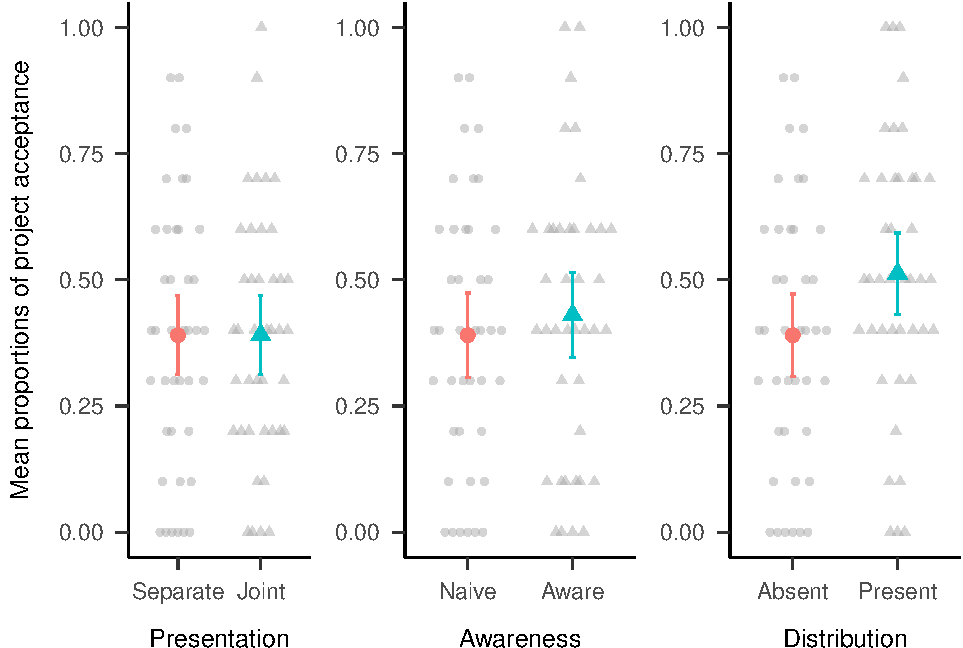
\includegraphics[width=1\linewidth]{effect-of-choice-bracketing-on-risk-aggregation_files/figure-latex/plot-aggregation-2-proportion-1} \caption{Mean proportion of project acceptance for the presentation, awareness, and distribution effects. The condition on the left of each effect is the reference condition (separate presentation, naive awareness, distribution absent). As such, it is identical for the three effects. Error bars represent 95\% confidence intervals. Raw data are plotted in the background.}\label{fig:plot-aggregation-2-proportion}
\end{figure}

Further, as Figure~\ref{fig:plot-aggregation-2-choice-trials} shows, it
doesn't seem as if the previous awareness by trial effect was replicated.



\begin{figure}
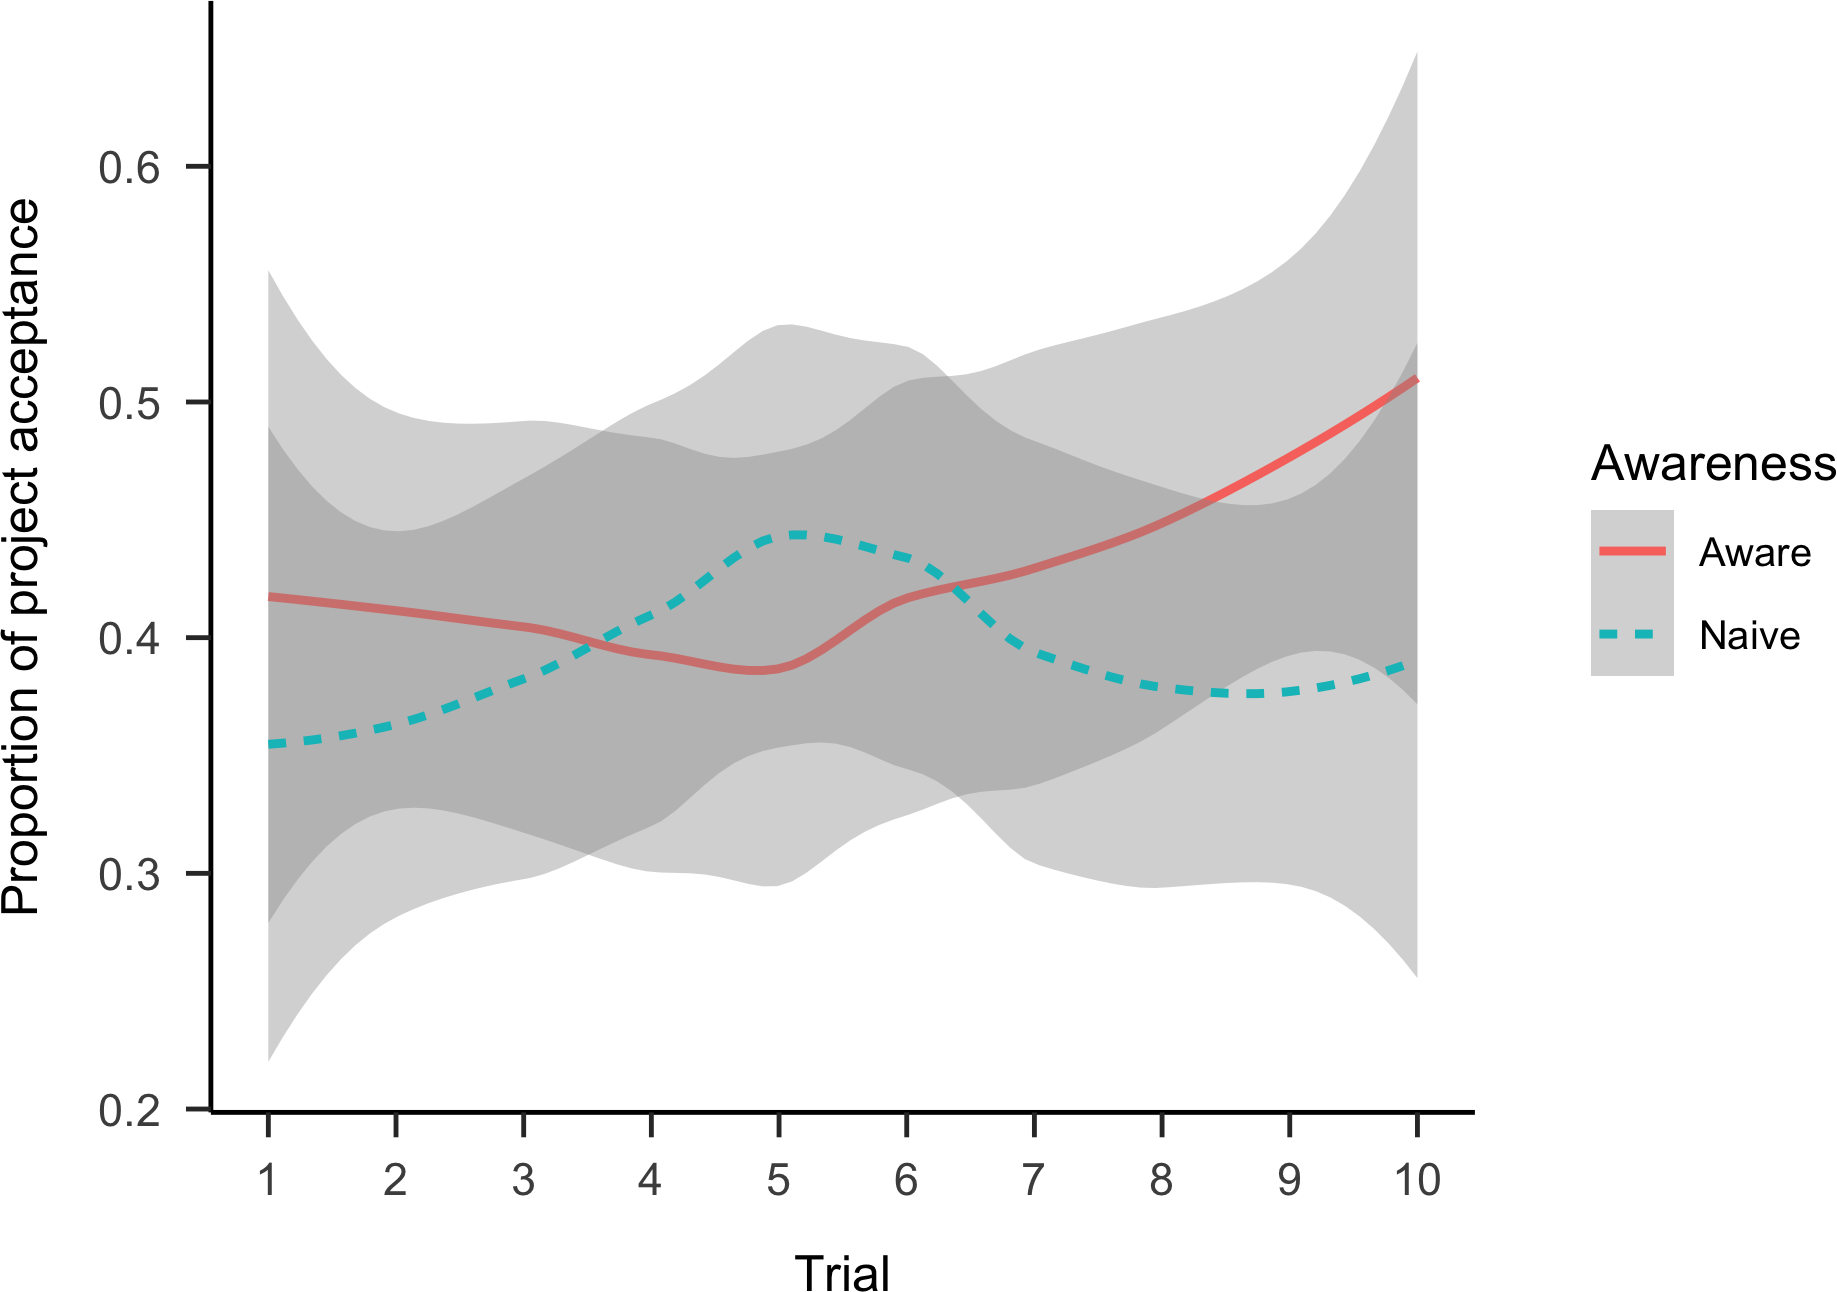
\includegraphics[width=1\linewidth]{effect-of-choice-bracketing-on-risk-aggregation_files/figure-latex/plot-aggregation-2-choice-trials-1} \caption{Mean project acceptance for separate presentation, distribution absent condition, by awareness and trial. LOESS method was used for smoothing over trials and the shading represents 95\% confidence intervals.}\label{fig:plot-aggregation-2-choice-trials}
\end{figure}

\hypertarget{follow-up}{%
\paragraph{Follow-up}\label{follow-up}}

The portfolio choice data from both the number and binary questions were
congruent with the above, finding that those in the distribution condition were
more likely to invest (see Appendix~\ref{results-aggregation-2-appendix}).

\hypertarget{discussion-aggregation-4}{%
\subsubsection{Discussion}\label{discussion-aggregation-4}}

Experiment~2 found support for
Hypothesis~\ref{hyp:distribution-aggregation-2}. Seeing an outcome
distribution of a business project portfolio had a strong effect on
participants' decision-making. Participants indicated that they would invest in
more projects and were more likely to indicate that they would invest in the
entire portfolio. However, the awareness and presentation effects found in
Experiment~1 (see Section~\ref{results-aggregation-1}) did not replicate.

These findings provide evidence for choice bracketing. That is, people do seem
to be primarily considering gambles one at a time. Further, these findings
suggest that that the main bottleneck for appropriately aggregating a set of
gambles is a computational one. That is, people simply cannot mentally combine
the outcomes and probabilities in a way that sufficiently approximates the
outcome distribution display.

The lack of replication of the awareness and presentation effects provides
evidence against a naive aggregation account of the distribution effect.
Specifically this suggests that the distribution effect is a result of a lack of
ability to mathematically combine risk, rather than naive aggregation. If some
of the bottleneck was attributable to a lack of realisation that the individual
gambles could be grouped together, then the effects from Experiment~1 should
have replicated. Instead it seems that even when people have an opportunity to
consider an entire set of risky choices together (and consider that the gains
may outweigh the losses), they do not do this.

In Experiment~2, all the gambles came from the same domain. This was done to
attempt to replicate the relevant effects from Experiment~1. However, there
could have been something about that particular domain that led to the lack of
replication. A follow-up experiment addressed this issue by presenting
participants with 20 gambles from 10 different industries and still did not
replicate the awareness effect (see Appendix~\ref{aggregation-4}).

\hypertarget{general-discussion}{%
\subsection{General Discussion}\label{general-discussion}}

When making one decision about a series of risky choices, it is clear that
people have an intuitive sense of the advantages of risk aggregation (e.g., Samuelson, \protect\hyperlink{ref-samuelson1963}{1963}). However, because risky choices are typically made one at a time
in the real world, this chapter aimed to identify whether (and how) this
intuition could be leveraged in this more realistic scenario. Overall, there was
little evidence that subtle cues could tap into this intuitive advantage of risk
aggregation, and clear visualisations of outcome distributions were needed to
assist people's risk aggregation. This suggests that the act of deciding can
create a strong cognitive barrier to treating a series of decisions as if they
were one. However, as elaborated below, the success of the outcome distribution
for overcoming this cognitive barrier in the current paradigm is a novel and
important finding.

This chapter found that some choice bracketing facilitated risk aggregation in
description-based repeated-play gambles. This paradigm has never been a target
of research. Early work on risk aggregation involved multi-play gambles, which
treated gambles as simultaneous and identical. However, most risky choice
outside the lab involves considering multiple choices independently, as in
repeated-play paradigms. Most repeated-play paradigms have involved providing
participants with feedback, or allowing them to sample from outcome
distributions. Large real-life investments are different, as their outcomes are
not eventuated immediately (and do not allow for distribution sampling). The
limited prior work using description-based repeated-play gambles did not
consider the effect of choice bracketing on risk aggregation. As such, the
paradigm used in this chapter allowed for the investigation of choice bracketing
in a way that is more isomorphic with real-life prescriptions.

Experiment~1 found evidence for the effects of similarity, presentation, and
awareness of the number of projects. Experiment~2 found evidence for the effect
of an outcome distribution but did not replicate the presentation and awareness
effects. Subsequent follow up experiments (reported in
Appendices~\ref{aggregation-3} and~\ref{aggregation-4}) again tested the
similarity and awareness effects. These experiments found evidence for naive
diversification (an advantage for low similarity) when considering all projects
once and did not replicate the trial-by-trial interaction from Experiment~1.

Therefore, in addition to the novelty of the paradigm itself, this chapter found
that choice bracketing facilitates risk aggregation, if aided by the aggregated
distribution. As per Hypothesis~\ref{hyp:distribution-aggregation-2},
Experiment~2 found that showing a distribution of outcome probabilities without
inter-trial feedback reduced risk aversion. Further, there was mixed evidence
for Hypothesis~\ref{hyp:similarity-aggregation-1}, such that people were less
risk averse when the set of projects they saw were dissimilar, but only when
offered them as a portfolio (see Appendix~\ref{aggregation-3}). There was only
minimal evidence for Hypotheses~\ref{hyp:awareness-aggregation-1}
and~\ref{hyp:presentation-aggregation-1}, suggesting that viewing projects
together and an awareness of the number of projects are not sufficient to
encourage aggregation. Altogether, it seems that subtle contextual cues are
often not sufficient to encourage risk aggregation and that people need risk to
be is aggregated for them explicitly in order to understand the benefits of
aggregation.

\hypertarget{theoretical-implications}{%
\subsubsection{Theoretical Implications}\label{theoretical-implications}}

The finding that participants are less risk averse when provided with an
aggregated outcome distribution is congruent with previous work (e.g., Redelmeier \& Tversky, \protect\hyperlink{ref-redelmeier1992}{1992}). However, when distributions have been previously used, gambles
were identical---as in multi-play paradigms---and used immediate feedback for
repeated-play paradigms (e.g., Benartzi \& Thaler, \protect\hyperlink{ref-benartzi1999}{1999}). As mentioned previously, both
these paradigms have limited ecological validity because usually people are
faced with non-identical sequential choices and do not receive immediate
feedback. This work is the first to provide evidence for this aggregation effect
with non-identical gambles without feedback.

The other choice bracketing findings that showed little success with aiding
aggregation are less congruent with previous research. Sokol-Hessner et al. (\protect\hyperlink{ref-sokolhessner2009}{2009}) and
Sokol-Hessner et al. (\protect\hyperlink{ref-sokolhessner2012}{2012}) found that encouraging participants to make decisions akin to
a professional investor increased the amount of risky choices they made. The
results showed that a subtler manipulation---whether or not participants were
aware of the number of choices to be made---is not sufficient to encourage
aggregation. Hsee et al. (\protect\hyperlink{ref-hsee1999}{1999}) found that useful, but hard-to-interpret, attributes were
used more when the options were presented jointly, rather than separately. In
the case of these experiments, the ``hard to interpret'' element of the decision
set was the risk of the projects. Contrary to Hsee et al. (\protect\hyperlink{ref-hsee1999}{1999}), it seems that risk was
not always accounted for more when projects were presented jointly, rather than
separately. More study is needed to understand whether the effects that were
seen in Experiment~1 but not replicated in the subsequent experiments are due to
statistical chance or unexplored elements of the experiment.

Research on the effect of option similarity on choice (e.g., Markman \& Medin, \protect\hyperlink{ref-markman1995}{1995})
suggests that alignable differences are more important than non-alignable
differences. Further, the effects of multi-play gambles and outcome
distributions on risk aggregation are only seen when participants perceive the
options as fungible (e.g., DeKay \& Kim, \protect\hyperlink{ref-dekay2005}{2005}). As such, it was predicted that a set of
investments that involve the same type of investment would be seen as more
similar, and therefore be considered as fungible.
Hypothesis~\ref{hyp:similarity-aggregation-1} predicted that this would
facilitate a broad bracketing, and therefore more risk aggregation.

Instead, the results showed that choice similarity did not affect individual
project allocations. However, when participants were given an all-or-nothing
choice for the entire set of projects, those that viewed dissimilar projects
were more likely to take the entire set projects than those that viewed similar
projects. This is different from the initial hypothesis, however, it may still
suggest an effect of choice bracketing. That is, this effect was only found when
participants were asked about the entire portfolio of projects, rather than when
they had a chance to make a choice about each project. The way that the question
was framed may have acted to broadly bracket the choices by forcing the choice.

A diversified portfolio is one whose investments are uncorrelated or negatively
correlated. According to portfolio theory (Markowitz, \protect\hyperlink{ref-markowitz1952}{1952}), a diversified
portfolio is preferred to one that is not diversified, because it reduces the
probability of a loss. When some investments have losses, others will have
gains---the root of ``don't keep all your eggs in one basket.'' Typically,
questions of gamble aggregation assume that each gamble is independent. That is,
the gambles are uncorrelated. As such, aggregation of a portfolio already
assumes that the portfolio is somewhat diversified (or at least that the gambles
aren't perfectly correlated).

In the case of the similarity effect, the choice bracketing did not seem to
encourage aggregation, but instead appears to have encouraged a naive
diversification (Hedesstrom et al., \protect\hyperlink{ref-hedesstrom2006}{2006}; Read \& Loewenstein, \protect\hyperlink{ref-read1995}{1995}). It could not have been actual
diversification, because the projects did not contain correlational information.
Rather, participants could have been more eager to accept the project portfolio
due to the higher variability between projects (due to the similarity
manipulation).

This finding suggests that there may be trade-off between aggregation and
diversification. The literature shows that people prefer multi-play gambles to
single-play gambles. However, participants in this chapter were more likely to
aggregate diverse repeated-play gambles to similar repeated-play gambles when
these were bracketed broadly. Therefore, people are likely to still need choice
bracketing. That is, diverse repeated-play gambles that are not bracketed are
simply individual single-play gambles.

One way to test this explanation is by using identical gambles. This chapter
used unique gambles to increase ecological validity. However, the above
explanation would predict that participants prefer non-identical repeated-play
gambles to identical repeated-play gambles when these are bracketed. However,
when these gambles are not presented as a portfolio, it is likely that the
identical gambles would be preferred overall because the non-identical gambles
would be represented as individual single-play gambles.

It is also possible that similarity effects were not seen because the sequence
of gambles itself led to naive aggregation for all conditions. One way that this
could be tested is by interweaving other tasks in-between the gambles to break
them up. Then similarity may play a role by allowing bracketing across otherwise
distinct gambles. Multiple sets of gambles can be interweaved with similarity
alone creating the potential sets. The prediction is that without similarity the
gambles would not be aggregated.

\hypertarget{how-does-choice-bracketing-facilitate-aggregation}{%
\paragraph{How Does Choice Bracketing Facilitate Aggregation?}\label{how-does-choice-bracketing-facilitate-aggregation}}

Much of the literature (e.g., Benartzi \& Thaler, \protect\hyperlink{ref-benartzi1999}{1999}) is not clear about why choice
bracketing occurs. Some explain the effect of bracketing on aggregation using
risk aversion (e.g., Read et al., \protect\hyperlink{ref-read1999}{1999}), while others refer to the increased weighting
of potential losses (Webb \& Shu, \protect\hyperlink{ref-webb2017}{2017}).

Decision-from-experience \emph{sampling} studies explain the underweighting of rare
events (as opposed to the overweighting that occurs with
decisions-from-description) by sampling bias and recency effects (e.g., Hertwig et al., \protect\hyperlink{ref-hertwig2004}{2004}; Wulff et al., \protect\hyperlink{ref-wulff2018}{2018}). That is, they explain that people are less risk
averse for positive EV gambles because when they sample from the distribution
they only sample a small amount (usually approximately 20 times) so they do not
experience rare events very often. Also, the latter half of the sequence of
sampling is significantly more predictive than the former (recency effect). Some
decision-from-experience \emph{feedback} studies explain this effect by ``choice
inertia'' (Camilleri \& Newell, \protect\hyperlink{ref-camilleri2011}{2011}). That is, ``the tendency to repeat the last choice,
irrespective of the obtained outcome'' (p.~383). However, there is not much more
elaboration beyond this. Repeated-play gambles show more underweighting than
multi-play gambles. This is said to be due to a ``reliance on a very small set of
samples'' (Camilleri \& Newell, \protect\hyperlink{ref-camilleri2013}{2013}, p. 64). However, this explanation does not account for
repeated-play effects independently.

The experiments in this chapter shed some light about the mechanisms behind why
choice bracketing may affect risk aggregation in repeated-play gambles without
feedback. Two explanations were proposed: participants may realise that some
gains will offset the losses, or they may need explicit aggregation. Not finding
evidence for the subtle choice bracketing manipulations suggests that people do
not intuitively consider that the gains of their choices may offset the
potential losses. Perhaps the possibility of recouped losses would become more
salient when other participants are explicitly told of this possibility, as in
Sokol-Hessner et al. (\protect\hyperlink{ref-sokolhessner2009}{2009}). Their explicit instruction manipulation is introduced above
as appearing unrealistically strong, but the results of this chapter suggest
that people do need very explicit scaffolding in order to use risk aggregation.

\hypertarget{practical-implications}{%
\subsubsection{Practical Implications}\label{practical-implications}}

This research implies some prescriptions for capital allocation decision-making.
For instance, even if managers implement processes that encourage a joint
evaluation of projects, this may be insufficient to encourage aggregation.
Projects need to very explicitly be considered as individual components in a
portfolio in order to facilitate better risk aggregation. Some companies are
already implementing processes that make this more explicit (Lovallo et al., \protect\hyperlink{ref-lovallo2020}{2020}). This
is especially important for those that would still have to evaluate projects
separately. Further, this work shows the importance of being explicit about the
forecasted probabilities of project success. Doing this is necessary for the
aggregation process. Even more ideal would be to forecast project success using
an entire probability distribution for the different possible outcomes. However,
research shows that people struggle to construct such distributions (e.g., Alpert \& Raiffa, \protect\hyperlink{ref-alpert1982}{1982}; Schaefer \& Borcherding, \protect\hyperlink{ref-schaefer1973}{1973}; Staël von Holstein, \protect\hyperlink{ref-staelvonholstein1971}{1971}; Tversky \& Kahneman, \protect\hyperlink{ref-tversky1974}{1974}) and
Chapter~\ref{alignment} shows that people struggle to use such variance
information when making allocation decisions. Regardless, the benefits of risk
aggregation can be used even if forecast information is limited (e.g., only a
point estimate and a probability) and only one project is being considered.
Specifically, a proposed project can be seen in a larger context by aggregating
it with projects from the immediate past.

Interestingly, participants were less risk averse about a portfolio of projects
when industries differed, compared to when they were all from the same industry.
Simply manipulating the similarity of financially-irrelevant semantics of a set
of choices affected participants' risk aversion. This has implications for
managerial settings. Executives in multi-business firms often have to make
capital allocation decisions that involve comparing dissimilar projects. How can
an oil well exploration project be appropriately compared to an oil refinery? Or
to a microchip project? Chapter~\ref{alignment} suggests that evaluating
dissimilar business projects is more difficult to comparing similar projects.
The current work suggests that managers may actually be \emph{less} likely to realise
the benefits of aggregation when they are in a less diversified company. As
such, managers should complement an understanding of aggregation with that of
diversification. This might help to avoid being biased by a lack of variety of
projects despite a potentially high level of diversification.

\hypertarget{future-research}{%
\subsubsection{Future Research}\label{future-research}}

The main novelty of the experiments in this chapter comes from increasing
ecological validity of risky choice problems by removing inter-trial feedback.
Future work should test even more realistic scenarios. Such studies should
involve managers, ideally in multi-business firms. Investigating whether the
choice bracketing findings from these experiments replicates in a sample of
managers will help to determine whether these results could be applied to
real-world managerial decision-making. This is especially important since
Haigh and List (\protect\hyperlink{ref-haigh2005}{2005}) found that professional traders show more myopic loss aversion than
students. Further, the similarity, awareness, and presentation manipulations
should be tested with managers since it is possible that they have a greater
sense of naive aggregation and are therefore more likely to be more amenable to
such manipulations. The addition of extra payment for better performance on the
task might also assist in making the task more isomorphic with real-world
managerial decisions. Further, in the present experiments, participants viewed
the projects all in the space of one session. However, this is not completely
isomorphic to real life, where managers make many other decisions that are
unrelated to the large risky investments at their companies. Future research
should test participants over a longer period of time (as in Beshears et al., \protect\hyperlink{ref-beshears2016}{2016}) in
order to see whether the effects of the manipulations replicate in a more
realistic environment.

\newpage

\newpage

\hypertarget{references}{%
\section{References}\label{references}}

\setlength{\parindent}{-0.5in}
\setlength{\leftskip}{0.5in}

\hypertarget{refs}{}
\begin{cslreferences}
\leavevmode\hypertarget{ref-aloysius2007}{}%
Aloysius, J. A. (2007). Decision making in the short and long run: Repeated gambles and rationality. \emph{British Journal of Mathematical and Statistical Psychology}, \emph{60}(1), 61--69. \url{https://doi.org/10/czgkh3}

\leavevmode\hypertarget{ref-alpert1982}{}%
Alpert, M., \& Raiffa, H. (1982). A progress report on the training of probability assessors. In D. Kahneman, P. Slovic, \& A. Tversky (Eds.), \emph{Judgment under uncertainty} (pp. 294--305). Cambridge University Press. \url{https://doi.org/10.1017/CBO9780511809477.022}

\leavevmode\hypertarget{ref-barron2003}{}%
Barron, G., \& Erev, I. (2003). Small feedback-based decisions and their limited correspondence to description-based decisions. \emph{Journal of Behavioral Decision Making}, \emph{16}(3), 215--233. \url{https://doi.org/10/d3jsr8}

\leavevmode\hypertarget{ref-barron2010}{}%
Barron, G., \& Leider, S. (2010). The role of experience in the Gambler's Fallacy. \emph{Journal of Behavioral Decision Making}, \emph{23}(1), 117--129. \url{https://doi.org/10/d3p92r}

\leavevmode\hypertarget{ref-bellemare2005}{}%
Bellemare, C., Krause, M., Kröger, S., \& Zhang, C. (2005). Myopic loss aversion: Information feedback vs. Investment flexibility. \emph{Economics Letters}, \emph{87}(3), 319--324. \url{https://doi.org/10/dfjq7n}

\leavevmode\hypertarget{ref-benartzi1999}{}%
Benartzi, S., \& Thaler, R. H. (1999). Risk Aversion or Myopia? Choices in Repeated Gambles and Retirement Investments. \emph{Management Science}, \emph{45}(3), 364--381. \url{https://doi.org/10/cjhp6t}

\leavevmode\hypertarget{ref-beshears2016}{}%
Beshears, J., Choi, J. J., Laibson, D., \& Madrian, B. C. (2016). Does Aggregated Returns Disclosure Increase Portfolio Risk Taking? \emph{The Review of Financial Studies}, \emph{30}(6), 1971--2005. \url{https://doi.org/10/gjscs7}

\leavevmode\hypertarget{ref-bjornsen2019}{}%
Bjørnsen, K., \& Aven, T. (2019). Risk aggregation: What does it really mean? \emph{Reliability Engineering \& System Safety}, \emph{191}, 106524. \url{https://doi.org/10/gjscst}

\leavevmode\hypertarget{ref-bristow2011}{}%
Bristow, R. E. (2011). \emph{There is more to Life than Expected Values: Results of Free Distributions of Multiple-Play Gambles} {[}Masters thesis, Miami University{]}. \url{https://etd.ohiolink.edu/apexprod/rws_etd/send_file/send?accession=miami1304352729}

\leavevmode\hypertarget{ref-camilleri2013}{}%
Camilleri, A. R., \& Newell, B. R. (2013). The long and short of it: Closing the description-experience ``gap'' by taking the long-run view. \emph{Cognition}, \emph{126}(1), 54--71. \url{https://doi.org/10/f4gq3w}

\leavevmode\hypertarget{ref-camilleri2011}{}%
Camilleri, A. R., \& Newell, B. R. (2011). When and why rare events are underweighted: A direct comparison of the sampling, partial feedback, full feedback and description choice paradigms. \emph{Psychonomic Bulletin \& Review}, \emph{18}(2), 377--384. \url{https://doi.org/10/cz55xk}

\leavevmode\hypertarget{ref-coombs1971}{}%
Coombs, C. H., \& Bowen, J. N. (1971). A test of VE-theories of risk and the effect of the central limit theorem. \emph{Acta Psychologica}, \emph{35}(1), 15--28. \url{https://doi.org/10/dm5gbv}

\leavevmode\hypertarget{ref-dekay2011}{}%
DeKay, M. L. (2011). Are Medical Outcomes Fungible? A Survey of Voters, Medical Administrators, and Physicians. \emph{Medical Decision Making}, \emph{31}(2), 338--353. \url{https://doi.org/10/b539tb}

\leavevmode\hypertarget{ref-dekay2006}{}%
DeKay, M. L., Hershey, J. C., Spranca, M. D., Ubel, P. A., \& Asch, D. A. (2006). Are medical treatments for individuals and groups like single-play and multiple-play gambles? \emph{Judgment and Decision Making}, \emph{1}(2), 12. \url{http://journal.sjdm.org/jdm06133.pdf}

\leavevmode\hypertarget{ref-dekay2005}{}%
DeKay, M. L., \& Kim, T. G. (2005). When things don't add up: The role of perceived fungibility in repeated-play decisions. \emph{Psychological Science}, \emph{16}(9), 667--672. \url{https://doi.org/10/ddgt5v}

\leavevmode\hypertarget{ref-ert2013}{}%
Ert, E., \& Erev, I. (2013). On the descriptive value of loss aversion in decisions under risk: Six clarifications. \emph{Judgment and Decision Making}, \emph{8}(3), 22. \url{http://journal.sjdm.org/12/12712/jdm12712.pdf}

\leavevmode\hypertarget{ref-gneezy1997}{}%
Gneezy, U., \& Potters, J. (1997). An Experiment on Risk Taking and Evaluation Periods. \emph{The Quarterly Journal of Economics}, \emph{112}(2), 631--645. \url{https://doi.org/10/bpkbhz}

\leavevmode\hypertarget{ref-haigh2005}{}%
Haigh, M. S., \& List, J. A. (2005). Do Professional Traders Exhibit Myopic Loss Aversion? An Experimental Analysis. \emph{The Journal of Finance}, \emph{60}(1), 523--534. \url{https://doi.org/10/c7jn9k}

\leavevmode\hypertarget{ref-haisley2008}{}%
Haisley, E., Mostafa, R., \& Loewenstein, G. (2008). Myopic risk-seeking: The impact of narrow decision bracketing on lottery play. \emph{Journal of Risk and Uncertainty}, \emph{37}(1), 57--75. \url{https://doi.org/10/czj8x7}

\leavevmode\hypertarget{ref-hedesstrom2006}{}%
Hedesstrom, T. M., Svedsater, H., \& Garling, T. (2006). Covariation neglect among novice investors. \emph{Journal of Experimental Psychology}, \emph{12}(3), 155--165. \url{https://doi.org/10/ftmd77}

\leavevmode\hypertarget{ref-hertwig2004}{}%
Hertwig, R., Barron, G., Weber, E. U., \& Erev, I. (2004). Decisions from experience and the effect of rare events in risky choice. \emph{Psychological Science}, \emph{15}(8), 534--539. \url{https://doi.org/10/b274n8}

\leavevmode\hypertarget{ref-hsee1999}{}%
Hsee, C. K., Loewenstein, G. F., Blount, S., \& Bazerman, M. H. (1999). Preference reversals between joint and separate evaluations of options: A review and theoretical analysis. \emph{Psychological Bulletin}, \emph{125}(5), 576--590. \url{https://doi.org/10/dm3fvc}

\leavevmode\hypertarget{ref-jessup2008}{}%
Jessup, R. K., Bishara, A. J., \& Busemeyer, J. R. (2008). Feedback Produces Divergence From Prospect Theory in Descriptive Choice. \emph{Psychological Science}, \emph{19}(10), 1015--1022. \url{https://doi.org/10/bgb3qs}

\leavevmode\hypertarget{ref-joag1990}{}%
Joag, S. G., Mowen, J. C., \& Gentry, J. W. (1990). Risk perception in a simulated industrial purchasing task: The Effects of single versus multi-play decisions. \emph{Journal of Behavioral Decision Making}, \emph{3}(2), 91--108. \url{https://doi.org/10/czwknv}

\leavevmode\hypertarget{ref-kahneman1993}{}%
Kahneman, D., \& Lovallo, D. (1993). Timid Choices and Bold Forecasts: A Cognitive Perspective on Risk Taking. \emph{Management Science}, \emph{39}(1), 17--31. \url{https://doi.org/10/c8vntn}

\leavevmode\hypertarget{ref-kahneman1979}{}%
Kahneman, D., \& Tversky, A. (1979). Prospect Theory: An Analysis of Decision under Risk. \emph{Econometrica}, \emph{47}(2), 263--291. \url{https://doi.org/10/g98}

\leavevmode\hypertarget{ref-keren1991}{}%
Keren, G. (1991). Additional tests of utility theory under unique and repeated conditions. \emph{Journal of Behavioral Decision Making}, \emph{4}(4), 297--304. \url{https://doi.org/10/bqqkt4}

\leavevmode\hypertarget{ref-keren1987}{}%
Keren, G., \& Wagenaar, W. A. (1987). Violation of utility theory in unique and repeated gambles. \emph{Journal of Experimental Psychology: Learning, Memory, and Cognition}, \emph{13}(3), 387. \url{https://doi.org/10/dkr96j}

\leavevmode\hypertarget{ref-klos2013}{}%
Klos, A. (2013). Myopic loss aversion: Potential causes of replication failures. \emph{Judgment and Decision Making}, \emph{8}(5), 13. \url{http://journal.sjdm.org/12/121229/jdm121229.pdf}

\leavevmode\hypertarget{ref-klos2005}{}%
Klos, A., Weber, E. U., \& Weber, M. (2005). Investment Decisions and Time Horizon: Risk Perception and Risk Behavior in Repeated Gambles. \emph{Management Science}, \emph{51}(12), 1777--1790. \url{https://doi.org/10/bbrvhd}

\leavevmode\hypertarget{ref-koehler1994}{}%
Koehler, J. J., Gibbs, B. J., \& Hogarth, R. M. (1994). Shattering the illusion of control: Multi-shot versus single-shot gambles. \emph{Journal of Behavioral Decision Making}, \emph{7}(3), 183--191. \url{https://doi.org/10/fwmwjs}

\leavevmode\hypertarget{ref-langer2001}{}%
Langer, T., \& Weber, M. (2001). Prospect Theory, Mental Accounting, and Differences in Aggregated and Segregated Evaluation of Lottery Portfolios. \emph{Management Science}, \emph{47}(5), 716--733. \url{https://doi.org/10/fcfk69}

\leavevmode\hypertarget{ref-li2003}{}%
Li, S. (2003). The role of Expected Value illustrated in decision-making under risk: Single-play vs multiple-play. \emph{Journal of Risk Research}, \emph{6}(2), 113--124. \url{https://doi.org/10/cz6phv}

\leavevmode\hypertarget{ref-liu2009}{}%
Liu, H.-H., \& Colman, A. M. (2009). Ambiguity aversion in the long run: Repeated decisions under risk and uncertainty. \emph{Journal of Economic Psychology}, \emph{30}(3), 277--284. \url{https://doi.org/10/d5p9kw}

\leavevmode\hypertarget{ref-lopes1996}{}%
Lopes, L. L. (1996). When Time Is of the Essence: Averaging, Aspiration, and the Short Run. \emph{Organizational Behavior and Human Decision Processes}, \emph{65}(3), 179--189. \url{https://doi.org/10/fdtw45}

\leavevmode\hypertarget{ref-lovallo2020}{}%
Lovallo, D., Koller, T., Uhlaner, R., \& Kahneman, D. (2020). Your Company Is Too Risk-Averse. \emph{Harvard Business Review}, \emph{98}(2), 104--111.

\leavevmode\hypertarget{ref-ludvig2011}{}%
Ludvig, E. A., \& Spetch, M. L. (2011). Of Black Swans and Tossed Coins: Is the Description-Experience Gap in Risky Choice Limited to Rare Events? \emph{PLoS ONE}, \emph{6}(6), e20262. \url{https://doi.org/10/ds5q2k}

\leavevmode\hypertarget{ref-maccrimmon1986}{}%
MacCrimmon, K. R., Wehrung, D. A., \& Stanbury, W. T. (1986). \emph{Taking risks: The management of uncertainty} (pp. xv, 380). Free Press.

\leavevmode\hypertarget{ref-march1987}{}%
March, J. G., \& Shapira, Z. (1987). Managerial Perspectives on Risk and Risk Taking. \emph{Management Science}, \emph{33}(11), 1404--1418. \url{https://doi.org/10/ft2phq}

\leavevmode\hypertarget{ref-markman2010}{}%
Markman, A. B., \& Loewenstein, J. (2010). Structural comparison and consumer choice. \emph{Journal of Consumer Psychology}, \emph{20}(2), 126--137. \url{https://doi.org/10/d7b49c}

\leavevmode\hypertarget{ref-markman1995}{}%
Markman, A. B., \& Medin, D. L. (1995). Similarity and Alignment in Choice. \emph{Organizational Behavior and Human Decision Processes}, \emph{63}(2), 117--130. \url{https://doi.org/10/c8z7r9}

\leavevmode\hypertarget{ref-markowitz1952}{}%
Markowitz, H. (1952). Portfolio Selection. \emph{The Journal of Finance}, \emph{7}(1), 77--91. \url{https://doi.org/10/bhzd}

\leavevmode\hypertarget{ref-moher2010}{}%
Moher, E., \& Koehler, D. J. (2010). Bracketing effects on risk tolerance: Generalizability and underlying mechanisms. \emph{Judgment and Decision Making}, \emph{5}(5), 8. \url{http://journal.sjdm.org/10/10422/jdm10422.pdf}

\leavevmode\hypertarget{ref-montgomery1982}{}%
Montgomery, H., \& Adelbratt, T. (1982). Gambling decisions and information about expected value. \emph{Organizational Behavior and Human Performance}, \emph{29}(1), 39--57. \url{https://doi.org/10/cvgjp4}

\leavevmode\hypertarget{ref-rabin2009}{}%
Rabin, M., \& Weizsäcker, G. (2009). Narrow Bracketing and Dominated Choices. \emph{American Economic Review}, \emph{99}(4), 1508--1543. \url{https://doi.org/10/fk4rmz}

\leavevmode\hypertarget{ref-read1995}{}%
Read, D., \& Loewenstein, G. (1995). Diversification bias: Explaining the discrepancy in variety seeking between combined and separated choices. \emph{Journal of Experimental Psychology: Applied}, \emph{1}(1), 34. \url{https://doi.org/10/fcgvrw}

\leavevmode\hypertarget{ref-read1999}{}%
Read, D., Loewenstein, G., \& Rabin, M. (1999). Choice Bracketing. \emph{Journal of Risk and Uncertainty}, \emph{19}(1), 171--197. \url{https://doi.org/10/dh3rmv}

\leavevmode\hypertarget{ref-redelmeier1992}{}%
Redelmeier, D. A., \& Tversky, A. (1992). On the Framing of Multiple Prospects. \emph{Psychological Science}, \emph{3}(3), 191--193. \url{https://doi.org/10/ctw2k6}

\leavevmode\hypertarget{ref-ross1999}{}%
Ross, S. A. (1999). Adding Risks: Samuelson's Fallacy of Large Numbers Revisited. \emph{The Journal of Financial and Quantitative Analysis}, \emph{34}(3), 323--339. \url{https://doi.org/10/bj6r8r}

\leavevmode\hypertarget{ref-samuelson1963}{}%
Samuelson, P. A. (1963). Risk and Uncertainty: A Fallacy of Large Numbers. \emph{Scientia}, \emph{57}(98), 108--113. \url{https://www.casact.org/sites/default/files/database/forum_94sforum_94sf049.pdf}

\leavevmode\hypertarget{ref-schaefer1973}{}%
Schaefer, R. E., \& Borcherding, K. (1973). The assessment of subjective probability distributions: A training experiment. \emph{Acta Psychologica}, \emph{37}(2), 117--129. \url{https://doi.org/10/dpzkfb}

\leavevmode\hypertarget{ref-sokolhessner2012}{}%
Sokol-Hessner, P., Camerer, C. F., \& Phelps, E. A. (2012). Emotion regulation reduces loss aversion and decreases amygdala responses to losses. \emph{Social Cognitive and Affective Neuroscience}, \emph{8}(3), 341--350. \url{https://doi.org/10/fx5cn6}

\leavevmode\hypertarget{ref-sokolhessner2009}{}%
Sokol-Hessner, P., Hsu, M., Curley, N. G., Delgado, M. R., Camerer, C. F., \& Phelps, E. A. (2009). Thinking like a trader selectively reduces individuals' loss aversion. \emph{Proceedings of the National Academy of Sciences}, \emph{106}(13), 5035--5040. \url{https://doi.org/10/fhdrcw}

\leavevmode\hypertarget{ref-staelvonholstein1971}{}%
Staël von Holstein, C.-A. S. (1971). Two techniques for assessment of subjective probability distributions --- An experimental study. \emph{Acta Psychologica}, \emph{35}(6), 478--494. \url{https://doi.org/10/fgg6jn}

\leavevmode\hypertarget{ref-stutzer2013}{}%
Stutzer, M. (2013). Misperceptions of long-term investment performance Insights from an experiment. \emph{The Journal of Behavioral Finance \& Economics}, \emph{3}(1), 1--20. \url{http://www.aobf.org/wp-content/uploads/2020/06/1-Stutzer-and-Grant.pdf}

\leavevmode\hypertarget{ref-su2013}{}%
Su, Y., Rao, L.-L., Sun, H.-Y., Du, X.-L., Li, X., \& Li, S. (2013). Is making a risky choice based on a weighting and adding process? An eye-tracking investigation. \emph{Journal of Experimental Psychology: Learning, Memory, and Cognition}, \emph{39}(6), 1765--1780. \url{https://doi.org/10/gjscr2}

\leavevmode\hypertarget{ref-swalm1966}{}%
Swalm, R. O. (1966). Utility Theory--Insights into Risk Taking. \emph{Harvard Business Review}, \emph{44}(6), 123--136.

\leavevmode\hypertarget{ref-thaler1999}{}%
Thaler, R. H. (1999). Mental accounting matters. \emph{Journal of Behavioral Decision Making}, \emph{12}(3), 183--206. \url{https://doi.org/10/d4njp3}

\leavevmode\hypertarget{ref-thaler1997}{}%
Thaler, R. H., Tversky, A., Kahneman, D., \& Schwartz, A. (1997). The Effect of Myopia and Loss Aversion on Risk Taking: An Experimental Test. \emph{The Quarterly Journal of Economics}, \emph{112}(2), 647--661. \url{https://doi.org/10/fcf346}

\leavevmode\hypertarget{ref-tversky1981}{}%
Tversky, A., \& Kahneman, D. (1981). The framing of decisions and the psychology of choice. \emph{Science}, \emph{211}(4481), 453--458. \url{https://doi.org/10/fj3z3r}

\leavevmode\hypertarget{ref-tversky1974}{}%
Tversky, A., \& Kahneman, D. (1974). Judgment under Uncertainty: Heuristics and Biases. \emph{Science}, \emph{185}(4157), 1124--1131. \url{https://doi.org/10/gwh}

\leavevmode\hypertarget{ref-tversky1992}{}%
Tversky, A., \& Kahneman, D. (1992). Advances in prospect theory: Cumulative representation of uncertainty. \emph{Journal of Risk and Uncertainty}, \emph{5}(4), 297--323. \url{https://doi.org/10/cb57hk}

\leavevmode\hypertarget{ref-venkatraman2006}{}%
Venkatraman, S., Aloysius, J. A., \& Davis, F. D. (2006). Multiple prospect framing and decision behavior: The mediational roles of perceived riskiness and perceived ambiguity. \emph{Organizational Behavior and Human Decision Processes}, \emph{101}(1), 59--73. \url{https://doi.org/10/dszh5v}

\leavevmode\hypertarget{ref-webb2017}{}%
Webb, E. C., \& Shu, S. B. (2017). Is broad bracketing always better? How broad decision framing leads to more optimal preferences over repeated gambles. \emph{Judgment and Decision Making}, \emph{12}(4), 382. \url{http://journal.sjdm.org/17/17317/jdm17317.pdf}

\leavevmode\hypertarget{ref-wedell1994}{}%
Wedell, D. H., \& Bockenholt, U. (1994). Contemplating Single versus Multiple Encounters of a Risky Prospect. \emph{The American Journal of Psychology}, \emph{107}(4), 499. \url{https://doi.org/10/b4fs2p}

\leavevmode\hypertarget{ref-wedell1990}{}%
Wedell, D. H., \& Böckenholt, U. (1990). Moderation of preference reversals in the long run. \emph{Journal of Experimental Psychology: Human Perception and Performance}, \emph{16}(2), 429--438. \url{https://doi.org/10/bmn8hf}

\leavevmode\hypertarget{ref-wulff2018}{}%
Wulff, D. U., Mergenthaler-Canseco, M., \& Hertwig, R. (2018). A meta-analytic review of two modes of learning and the description-experience gap. \emph{Psychological Bulletin}, \emph{144}(2), 140--176. \url{https://doi.org/10/gc2s4c}

\leavevmode\hypertarget{ref-zeisberger2020}{}%
Zeisberger, S. (2020). \emph{Do People Care About Loss Probabilities?} \url{https://ssrn.com/abstract=2169394}
\end{cslreferences}


\end{document}
